%% The first command in your LaTeX source must be the \documentclass command.
\documentclass[manuscript]{acmart}
%% \BibTeX command to typeset BibTeX logo in the docs
\AtBeginDocument{%
  \providecommand\BibTeX{{%
    \normalfont B\kern-0.5em{\scshape i\kern-0.25em b}\kern-0.8em\TeX}}}
%% Rights management information.  This information is sent to you
%% when you complete the rights form.  These commands have SAMPLE
%% values in them; it is your responsibility as an author to replace
%% the commands and values with those provided to you when you
%% complete the rights form.
\copyrightyear{2020}
\acmYear{2020}
\setcopyright{acmcopyright}\acmConference[RecSys '20]{Fourteenth ACM Conference on Recommender Systems}{September 22--26, 2020}{Virtual Event, Brazil}
\acmBooktitle{Fourteenth ACM Conference on Recommender Systems (RecSys '20), September 22--26, 2020, Virtual Event, Brazil}
\acmPrice{15.00}
\acmDOI{10.1145/3383313.3412216}
\acmISBN{978-1-4503-7583-2/20/09}

% for float positioning
% Alter some LaTeX defaults for better treatment of figures:
    % See p.105 of "TeX Unbound" for suggested values.
    % See pp. 199-200 of Lamport's "LaTeX" book for details.
    %   General parameters, for ALL pages:
    \renewcommand{\topfraction}{0.9}	% max fraction of floats at top
    \renewcommand{\bottomfraction}{0.8}	% max fraction of floats at bottom
    %   Parameters for TEXT pages (not float pages):
    \setcounter{topnumber}{1}
    \setcounter{bottomnumber}{2}
    \setcounter{totalnumber}{4}     % 2 may work better
    \setcounter{dbltopnumber}{1}    % for 2-column pages
    \renewcommand{\dbltopfraction}{0.9}	% fit big float above 2-col. text
    \renewcommand{\textfraction}{0.07}	% allow minimal text w. figs
    %   Parameters for FLOAT pages (not text pages):
    \renewcommand{\floatpagefraction}{0.7}	% require fuller float pages
	% N.B.: floatpagefraction MUST be less than topfraction !!
    \renewcommand{\dblfloatpagefraction}{0.7}	% require fuller float pages

	% remember to use [htp] or [htpb] for placement

%% package import location??
\usepackage{multirow}
%\usepackage{amsmath}
\usepackage{graphicx}
\usepackage{stfloats}
%\usepackage{float}
%\restylefloat{table}

\begin{document}
%%
%% The "title" command has an optional parameter,
%% allowing the author to define a "short title" to be used in page headers.
\title[MEANTIME]{MEANTIME: Mixture of Attention Mechanisms with Multi-temporal Embeddings for Sequential Recommendation}
%\subtitle{My Subtitle}

%%
%% The "author" command and its associated commands are used to define
%% the authors and their affiliations.
%% Of note is the shared affiliation of the first two authors, and the
%% "authornote" and "authornotemark" commands
%% used to denote shared contribution to the research.

%\authornote{First Author Note}
%\orcid{1234-5678-9012}
%\authornotemark[1]
%\affiliation{
%  \institution{Seoul National University}
%  \streetaddress{Street}
%  \city{City}
%  \state{State}
%  \postcode{Postcode}
%}

\author{Sung Min Cho}
\affiliation{
  \institution{Seoul National University}
}
\email{tjdals4565@gmail.com}


\author{Eunhyeok Park}
\affiliation{
  \institution{POSTECH}
}
\email{canusglow@gmail.com}

\author{Sungjoo Yoo}
\affiliation{
  \institution{Neural Processing Research Center}
}
\affiliation{
  \institution{Seoul National University}
}
\email{sungjoo.yoo@gmail.com}

%%
%% By default, the full list of authors will be used in the page
%% headers. Often, this list is too long, and will overlap
%% other information printed in the page headers. This command allows
%% the author to define a more concise list
%% of authors' names for this purpose.
\renewcommand{\shortauthors}{Sung Min Cho, Eunhyeok Park, and Sungjoo Yoo}

%%
%% The abstract is a short summary of the work to be presented in the
%% article.
\begin{abstract}
Recently, self-attention based models have achieved state-of-the-art performance in sequential recommendation task. Following the custom from language processing, most of these models rely on a simple positional embedding to exploit the sequential nature of the user's history. However, there are some limitations regarding the current approaches. First, sequential recommendation is different from language processing in that timestamp information is available. Previous models have not made good use of it to extract additional contextual information. Second, using a simple embedding scheme can lead to information bottleneck since the same embedding has to represent all possible contextual biases. Third, since previous models use the same positional embedding in each attention head, they can wastefully learn overlapping patterns. To address these limitations, we propose MEANTIME (MixturE of AtteNTIon mechanisms with Multi-temporal Embeddings) which employs multiple types of temporal embeddings designed to capture various patterns from the user's behavior sequence, and an attention structure that fully leverages such diversity. Experiments on real-world data show that our proposed method outperforms current state-of-the-art sequential recommendation methods, and we provide an extensive ablation study to analyze how the model gains from the diverse positional information.
\end{abstract}

%%
%% The code below is generated by the tool at http://dl.acm.org/ccs.cfm.
%% Please copy and paste the code instead of the example below.
%%
\begin{CCSXML}
<ccs2012>
   <concept>
       <concept_id>10002951.10003317.10003338</concept_id>
       <concept_desc>Information systems~Retrieval models and ranking</concept_desc>
       <concept_significance>500</concept_significance>
       </concept>
 </ccs2012>
\end{CCSXML}

\ccsdesc[500]{Information systems~Retrieval models and ranking}
%%
%% Keywords. The author(s) should pick words that accurately describe
%% the work being presented. Separate the keywords with commas.
\keywords{Sequential Recommendation, Self-attention, Temporal Embedding, BERT}


%%
%% This command processes the author and affiliation and title
%% information and builds the first part of the formatted document.
\maketitle

\section{Introduction}
%(Paragraph 1: Explain sequential recommendation.)
%Capturing users' preferences from their history is essential for making effective recommendations. Traditional methods, such as Collaborative Filtering (CF), focus on modeling the relationship between users and items based only on their interaction history without considering the temporal information. However, temporal information is essential because users' preferences and items' characteristics might evolve over time. Furthermore, users' preferences might depend heavily on the context (e.g. one is likely to be interested in buying a keyboard after purchasing a desktop). Therefore, sequential recommendation aims to model the sequences of users' past behaviors to predict the next set of items that they are likely to prefer.

Capturing users' preferences from their history is essential for making effective recommendations, because users' preferences and items' characteristics are both dynamic. Furthermore, users' preferences depend heavily on the context (e.g., one is likely to be interested in buying a keyboard after purchasing a desktop). Therefore, sequential recommendation aims to predict the next set of items that users are likely to prefer by exploiting their history.


%Paragraph 2: Brief touch on recent methods. Finish with SASRec, TiSASRec? and BERT4Rec.
%There have been many attempts to apply various algorithms to better understand the sequential behaviors of users. Works such as \cite{rendle2010factorizing, SIMILARITYMC, MCAULEYMC2016, MCAULEYMC2017, he2016fusing} employed Markov-Chain models by assuming that users' behaviors depend solely on their last N behaviors. Some tried to incorporate time information in the traditional factorization methods \cite{TIMESVD++}. More recent works adopted deep learning techniques such as RNN~\cite{GRU4Rec, hidasi2018recurrent, RNN4Rec, HIERARCHICALGRU4REC, DREAM, wu2017recurrent, wu2017sequential, DINEVOLUTION}, CNN~\cite{CASER, CNNGENERATIVE, HIERARCHICALCNN}, GNN~\cite{SESSIONGNN} for sequence modeling. Especially, the latest success came from self-attention mechanisms. For example, SASRec~\cite{SASRec} designed a strong model that runs entirely on self-attention blocks. As more recent work, BERT4Rec~\cite{BERT4Rec} improved SASRec~\cite{SASRec} by replacing their model with BERT~\cite{BERT}, which was originally a huge success in NLP area.

%Paragraph 3: Point out the limitations of recent methods.
%Many algorithms have been tried to better understand the sequential behaviors of users~\cite{SASRec, BERT4Rec, hidasi2018recurrent, CASER, M3, rendle2010factorizing, DIN, MCAULEYMC2017}. Although these studies showed excellent performance, most of them use time information only to order the user's behaviors into a sequence. This can be considered a loss since we can embed time information to extract more patterns from the sequence. While recent works such as TiSASRec~\cite{TISASRec} successfully incorporated time information into their recommendation model, their usage of time was limited to a single embedding scheme. Assuming that adding novel positional embedding benefits performance, it is natural to investigate more forms of temporal encodings and a model architecture that can fully leverage such diversity.


Many algorithms have been proposed to better understand the sequential history of users~\cite{SASRec, BERT4Rec, hidasi2018recurrent, CASER, M3, rendle2010factorizing, DIN, TRANSREC}. Despite their excellent performance, most of them ignore the interactions' timestamp values. While recent works such as TiSASRec~\cite{TISASRec} successfully incorporated time information, their usage of time was also limited to a single embedding scheme. Since the timestamp values are rife with information, it would be beneficial to explore many forms of temporal embeddings that can fully extract diverse patterns, and model architectures that can fully leverage such diversity.



%Paragraph 4: Our solution.
%In this paper we propose \textbf{MEANTIME}(\textbf{M}ixtur\textbf{E} of \textbf{A}tte\textbf{NTI}on mechanisms with \textbf{M}ulti-temporal \textbf{E}mbeddings) to address the issues mentioned above.Recently, CTA\cite{CTA} demonstrated that using multiple kernels for modeling temporal influence can benefit performance. Inspired by this, \textbf{MEANTIME} introduces multiple temporal embeddings to better encode both absolute and relative positions of user-item interactions in a sequence. Moreover, we employ multiple self-attention blocks simultaneously to handle each positional encoding separately. This is profitable because each block can function as a sort of expert that focuses on a particular pattern of user behaviors. For example, one block could concentrate on short-term effects of nearby interactions, while another block could extract long-term effects from distant interactions. Some other blocks could disregard the positional bias, thereby only examining the relationship between items. Extensive experiments show that \textbf{MEANTIME} outperforms several state-of-the-art sequential recommendation algorithms on many real-world datasets.\\

In this paper we propose \textbf{MEANTIME} (\textbf{M}ixtur\textbf{E} of \textbf{A}tte\textbf{NTI}on mechanisms with \textbf{M}ulti-temporal \textbf{E}mbeddings) which introduces multiple temporal embeddings to better encode both absolute and relative positions of a user-item interaction in a sequence. Moreover, we employ multiple self-attention heads that handle each positional embedding separately. This is profitable because each head can play a role of expert that focuses on a particular pattern of user behaviors. 
%For example, one block could concentrate on short-term effects of nearby interactions, while another block could extract long-term effects from distant interactions. Some other blocks could disregard the positional bias, thereby only examining the relationship between items. 
Extensive experiments show that \textbf{MEANTIME} outperforms state-of-the-art algorithms on real-world datasets. Our contributions are as follows:
\begin{itemize}
\item We propose to diversify the embedding schemes that are used to encode the positions of user-item interactions in a sequence. This is done by applying multiple kernels to positions/values of timestamps in a sequence to create unique embedding matrices.
\item We also propose a novel model architecture that operates multiple self-attention heads simultaneously, where each head specializes in extracting certain patterns from the users' behaviors by utilizing one of the positional embeddings we propose above.
\item We conducted thorough experiments to show the effectiveness of our method on real-world datasets. We also provide a comprehensive ablation study that helps understand the effect of various components in our model.
\end{itemize}

% EH: Intro 1차 분량 조절 완료

%% RELATED WORK
\section{Related Work}
%\subsection{Self-Attention Mechanism}
%%Recently, a series of Transformer\cite{TRANSFORMER, TRANSFORMER-XL} based models \cite{BERT, XLNET}, which rely purely on multi-headed self-attention mechanism, have provided a strong basis for many tasks in language understanding. They also inspired many self-attention based sequential recommendation models such as SASRec\cite{SASRec} and BERT4Rec\cite{BERT4Rec}.
Given a stack of same-sized vectors, Transformer applies the following scaled dot-product attention:
\begin{displaymath}
  \textrm{Attention}(Q, K, V) = \textrm{softmax}(\frac{QK^T}{\sqrt{d}})V
\end{displaymath}
where $Q, K, V$ are queries, keys, and values each generated by separate linear projections applied to the same input vectors. Multi-headed self-attention differs from single-headed self-attention only in that it creates multiple sets of queries, keys, and values, each producing its own attention results which are concatenated in the final output. The capability of each query to assign more attention to relevant values makes it a powerful mechanism for understanding sequential data.

\subsection{Temporal Recommendation}
%When it comes to making relevant recommendations, time has always been an important factor for many reasons. For example, the characteristics of an item (e.g. popularity or relevance) can vary dramatically along with the time shift. Users are also heavily influenced by time since their interests continuously change and evolve over time. Furthermore, the temporal distance between the two interactions can tell a lot about their relationship. For these reasons, many works have tried to utilize time information effectively.

%TimeSVD++\cite{TIMESVD++}, which included time factor into the traditional matrix factorization method, was one of the main contributions for the winning of Netfliz Grand Prize \cite{NETFLIXPRIZE}. Bayesian Probabilistic Tensor Factorization (BPTF)\cite{BPTF} added time constraints when factorizing the tensors. However, these works were limited to the traditional factorization settings where the sequential information is ignored. Meanwhile, Time-LSTM\cite{TIMELSTM} equipped LSTMs with several forms of time gates to better model the time intervals in user's interaction sequence. Recently, CTA\cite{CTA} used temporal information crucially by using multiple parametrized kernel functions to calibrate the self-attention mechanism.


Since temporal information hold contextual information, they can be very crucial for recommendation performance. TimeSVD++ and BPTF~\cite{TIMESVD++, BPTF} adopted time factor into the matrix factorization method, and TimeSVD++ was one of the main contributions for the winning of Netflix Grand Prize~\cite{NETFLIXPRIZE}.
%Bayesian Probabilistic Tensor Factorization (BPTF)~\cite{BPTF} added time constraints when factorizing the tensors. However, these works were limited to the traditional factorization setting where the sequential nature of data is ignored. Meanwhile,
Time-LSTM~\cite{TIMELSTM} equipped LSTMs with several forms of time gates to better model the time intervals in user's interaction sequence. Recently, CTA~\cite{CTA} used multiple parametrized kernel functions on temporal information to calibrate the self-attention mechanism.

\subsection{Sequential Recommendation}
% Sequential recommendation aims to suggest relevant items based on the user's historical behaviors. Many algorithms have been deployed to better understand the sequential patterns of user's behaviors. Markov-chain based methods \cite{SIMILARITYMC, MCAULEYMC2016, MCAULEYMC2017, he2016fusing} use the traditional Markov Chain model by assuming that users' behaviors are affected only by their last few behaviors. FPMC \cite{rendle2010factorizing} merges Markov-chains with matrix factorization method for next-basket recommendation. Since the first suggestion by GRU4Rec\cite{GRU4Rec}, many RNN-based methods \cite{hidasi2018recurrent, RNN4Rec, HIERARCHICALGRU4REC, DREAM, wu2017recurrent, wu2017sequential, DINEVOLUTION} sought to bring the success of RNN in language understanding into item sequence understanding. To overcome the limitations of RNN models (namely, the strong order constraint imposed by RNN), CNN-based method CASER \cite{CASER}, and others\cite{CNNGENERATIVE, HIERARCHICALCNN} proposed to use CNNs to better capture the dependencies between items. Some works adopted GNN to understand user's session as a graph\cite{SESSIONGNN}.

Sequential recommendation aims to suggest relevant items based on the user's sequential history. Markov-chain based methods~\cite{SIMILARITYMC, MCAULEYMC2016, TRANSREC, he2016fusing} assume that users' behaviors are affected only by their last few behaviors. FPMC~\cite{rendle2010factorizing} merges Markov-chains with matrix factorization method for next-basket recommendation. Since the first suggestion by GRU4Rec~\cite{GRU4Rec}, many RNN-based methods~\cite{hidasi2018recurrent, RNN4Rec, HIERARCHICALGRU4REC, DREAM, wu2017recurrent, wu2017sequential, DINEVOLUTION} brought the success of RNN into item sequence understanding. To overcome the strong order constraint of RNN models, CNN-based methods~\cite{CASER, CNNGENERATIVE, HIERARCHICALCNN} were proposed. Some works adopted graph neural network (GNN) to understand user's session as a graph~\cite{SESSIONGNN}.

%As for attention mechanisms, NARM \cite{NARM}, STAMP \cite{STAMP}, etc incorporated vanilla attention mechanism with RNN. More recently, SASRec\cite{SASRec} successfully employed self-attention mechanism, which was a huge success in NLP areas\cite{TRANSFORMER, BERT, TRANSFORMER-XL, XLNET}. BERT4Rec \cite{BERT4Rec} improved SASRec by replacing their self-attention blocks with bi-directional transformers and using Cloze task to train the model. TiSASRec \cite{TISASRec} enhanced SASRec by merging timestamp information into self-attention operations. Our work seeks to further expand this trend by suggesting a novel model architecture that uses multiple types of positional embeddings and self-attention operations to better capture the diverse patterns in user's behaviors.

As for attention mechanisms, NARM~\cite{NARM} and STAMP~\cite{STAMP} incorporated vanilla attention mechanism with RNN. More recently, SASRec~\cite{SASRec} successfully employed self-attention mechanism, which was a huge success in NLP areas~\cite{TRANSFORMER, BERT, TRANSFORMER-XL, XLNET}. BERT4Rec~\cite{BERT4Rec} improved SASRec by adopting Transformer~\cite{TRANSFORMER} and Cloze-task based training method. TiSASRec~\cite{TISASRec} enhanced SASRec by merging timestamp information into self-attention operations. Our work seeks to further expand this trend by suggesting a novel model architecture that uses multiple types of temporal embeddings  and self-attention operations to better capture the diverse patterns in user's behaviors.

% EH: Relwork 1차 분량 조절 완료
% Transformer는 method에 합쳐서 한번에 설명하는게 좋을듯 

%% PROPOSED METHOD
\section{Proposed Method}
\begin{figure*}[t]
  \centering
  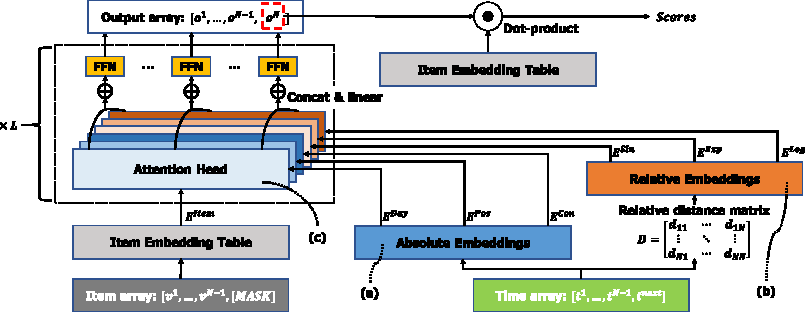
\includegraphics[width=0.9\linewidth]{figures/model_figure.pdf}
  \caption{Model Architecture}
  \Description[The figure describes our model architecture.]{In the figure, item array is converted by item embedding table and fed to each attention head. Time array is converted by absolute/relative embeddings into 6 different embeddings. Each attention head receives item embedding and unique temporal embedding. Concat&linear and FFN operation lies above the heads. Heads and FFNs are repeated for L layers. At the end of the layer, output vector is dot-producted with item embedding table to compute the final item score distribution.}
  \label{fig:model}
\end{figure*}

\begin{figure*}[t]
  \centering
  
\includegraphics[width=\linewidth]{figures/attention.pdf}
  \caption{Brief overview of single attention head in multi-headed attention structure. (a) absolute self-attention in Transformer (b) relative self-attention in Transformer-XL and MEANTIME (c) absolute self-attention in MEANTIME.}
  \Description[The figure describes three different types of single attention-head]{Figure(a) describes a single attention head used in transformer. The sum of E^Item and E^Pos is fed to the head. Figure(b) describes a single attention head from Transformer-xl and our model. E^Pos is replaced by E^R and positional information is not used in value computation. Linear layers are also separated between content and position. Figure(c) describes a single attention head used for absolute attention in our model. It borrows the structure from (a), but separates the content and position as in (b).}
  \label{fig:attntypes}
\end{figure*}

Several self-attention based recommendation models have been proposed recently~\cite{SASRec, BERT4Rec}. However, the positional factors have been rather overlooked in these models for many reasons. First, they don't utilize timestamp values which hold important contextual information. While TiSASRec~\cite{TISASRec} successfully addressed this issue, they also used a simple embedding scheme for temporal values. This can possibly lead to an information bottleneck since the same embedding has to represent all possible positional biases. Furthermore, since all attention heads use the same positional information, they might wastefully learn the same patterns. As a way to mitigate these problems, we devise a novel model architecture that injects various temporal embeddings for each attention head as shown in Figure \ref{fig:model}.

\subsection{Problem Formulation}
%Let $U=\{u_1,u_2,…,u_{|U|}\}$ be a set of users, and $V=\{v_1,v_2,…,v_{|V|}\}$ be a set of items. For each user $u \in U$, we have a sequence of items that the user interacted with in the past, denoted by $S_u=[v_1^{(u)},…,v_k^{(u)},…,v_{|S_u|}^{(u)}]$ where $v_k^{(u)}$ is the $k^{th}$ interacted item in chronological order. We also assume that each interaction is tagged by a positive integer which represents the absolute timestamp of the interaction (e.g. unix timestamp). Therefore each sequence $S_u$ has a corresponding time sequence $T_u=[t_1^{(u)},…,t_k^{(u)},…,t_{|S_u|}^{(u)}]$ where $t_k^{(u)}$ is the timestamp of $v_k^{(u)}$. Given an interaction history $(S_u,T_u)$ and a target timestamp $t_{|S_u |+1}^{(u)}$, our goal is to predict the next item that the user is likely to interact with at the target timestamp. This can be done by modeling the probability  $p\Big(v_{|S_u |+1}^{(u)} = v \Big| S_u,T_u \Big)$ over a set of candidate items for the user $u$ at timestamp $t_{|S_u|+1}^{(u)}$. 


Let $U$ be a set of users, and $V$ a set of items. For each user $u\in U$, we have a sequence of items $V^u=[v^u_1, ..., v^u_k, ..., v^u_{|V^u|}|v^u_k\in V]$ that the user previously interacted with in chronological order and the corresponding time sequence of the interaction $T^u=[t^u_1, ..., t^u_k, ..., t^u_{|V^u|}|t^u_k\in \mathbb{N}]$ that stores the absolute timestamp values.
%e.g., unix timestamp.
Our goal is to predict the next item $v^u_{next}$ that the user $u$ is likely to interact with at the target timestamp $t^u_{next}$ based on the given history $(V^u, T^u)$. % This can be done by modeling the probability  $p\Big(v_{|S_u |+1}^{(u)} = v \Big| S_u,T_u \Big)$ over a set of candidate items for the user $u$ at timestamp $t_{|S_u|+1}^{(u)}$. 

\sloppy Our model is based on a fixed-length model with length $N$ as in previous works~\cite{SASRec, BERT4Rec}. Given the history $(V_u, T_u)$ of user $u$, we feed $\mathbf{v} = [v^u_{|V^u|-N+2}, ..., v^u_{|V^u|}, \text{[MASK]}]$ and $\mathbf{t} = [t^u_{|V^u|-N+2}, ..., t^u_{|V^u|}, t^u_{next}]$ to the model. Then the model estimates $v_{next}$ as output. If the history is shorter than $N-1$, it is padded by a special token [PAD]. 


\subsection{Input Embedding}
\label{section:inputembedding}
The embedding layers convert $\mathbf{v}$ and $\mathbf{t}$ to hidden features that are provided to the attention module. In the case of item array $\mathbf{v}$, each element has an item index. This array is embedded as $E^{item} \in \mathbb{R}^ {N\times h}$ using the conventional look-up operation with a learnable item embedding table $M^I\in \mathbb{R}^{(|V|+1)\times h}$, where h is the hidden feature size. $M^I$ holds embeddings for $|V|$ items and [MASK] token.

In the case of $\mathbf{t}$, each element has a timestamp value.
%While previous studies~\cite{SASRec, BERT4Rec} use them only to impose an order on the sequence, these values actually hold a lot of information. For instance, temporal difference between two interactions is highly related to the influence they have on each other.
In previous studies, these values were embedded in a single embedding scheme, if they were used at all. However, given that user's behaviors are mixed with various patterns, a single embedding might not suffice. Moreover, using different encoding functions (instead of plain learnable values) for each embedding is beneficial since we can train each of them to learn a unique pattern. With these in mind, we propose six methods to embed $\mathbf{t}$: three absolute methods (Figure \ref{fig:model}(a)), and three relative methods (Figure \ref{fig:model}(b)).

Absolute embeddings encode each position in the sequence as $E^{Day}, E^{Pos}\text{, or } E^{Con} \in \mathbb{R}^{N \times h}$. The first is $\textbf{Day}$-embedding which converts the day of each timestamp into an embedding vector to get $E^{Day}$. We keep a learnable embedding matrix $M^D\in R^{|D|\times h}$ where $|D|$ is the number of possible days in the span of the dataset. In our analysis, $\textbf{Day}$ is a reasonable choice of time length considering the trade-off between matrix size and the effectiveness. $\textbf{Pos}$-embedding is analogous to the learnable positional embedding used in~\cite{BERT, BERT4Rec}, where each position has a corresponding embedding in $M^P\in R^{N\times h}$. We convert each position to get $E^{Pos}$. Note that in this case, the embeddings depend only on the indices of time array and not on the timestamp values. \textbf{Con}-embedding is similar to \textbf{Pos}-embedding, except that all position vectors are shared ($M^C\in R^{1\times h}$) to remove positional bias. Hence, $E^{Con}$ is a stack of repeated vectors.

Relative embeddings encode the relationship between each interaction pair in the sequence as $E^{Sin}, E^{Exp}\text{, or } E^{Log} \in \mathbb{R}^{N \times N \times h}$ by utilizing the temporal difference information. First, we define a matrix of temporal differences $\mathbf{D} \in \mathbb{R}^{N \times N}$ whose element is defined as $d_{ab} = (\mathbf{t}_a-\mathbf{t}_b)/\tau$, where $\tau$ is an adjustable unit time difference. We introduce three encoding functions for \textbf{D}.
%that capture different characteristics of these time intervals.
First, $\textbf{Sin}$ encoder converts the difference $d_{ab}$ to a hidden vector $\vec{\theta}_{ab} \in \mathbb{R}^{1 \times h}$, by the following equation:
\begin{equation}
    \vec{\theta}_{ab, 2c} = sin(\frac{d_{ab}}{freq^{\frac{2c}{h}}})\qquad\vec{\theta}_{ab, 2c+1} = cos(\frac{d_{ab}}{freq^{\frac{2c}{h}}})
\end{equation}
where $\vec{\theta}_{ab, c}$ is the $c^{th}$ value of the vector $\vec{\theta}_{ab}$ and $freq$ is an adjustable parameter.
%By applying the encoder function to $\mathbf{D}$, we get $E^{sinusoid} \in R^{N \times N \times h}$ as output.
Likewise, $\textbf{Exp}$ encoder and $\textbf{Log}$ encoder converts $d_{ab}$ to $\vec{e}_{ab}$ and $\vec{l}_{ab}$ respectively by applying the following equations:
\begin{equation}
  \vec{e}_{ab, c} = exp(\frac{-|d_{ab}|}{freq^{\frac{c}{h}}}) \qquad
  \vec{l}_{ab, c} = log(1 + \frac{|d_{ab}|}{freq^{\frac{c}{h}}})
\end{equation}
Stacking these vectors gives us $E^{Sin}, E^{Exp}$ and $E^{Log}$ respectively.

Each embedding offers a distinctive view on temporal data. For example, $\textbf{Sin}$ captures periodic occurrences. Larger time gap is either quickly decayed to zero in $\textbf{Exp}$ or manageably increased in $\textbf{Log}$. $\textbf{Day}$ can confine the attention scope within the same (or similar) day. $\textbf{Pos}$ can pick up the patterns learnt by the previous models. Finally, $\textbf{Con}$ removes positional bias altogether so that the attention can focus only on the relationship between items. These distinctive views enable our self-attention heads (Figure \ref{fig:model}(c)) to attend to different characteristics of the sequence.

\subsection{Self-Attention Structure}
\subsubsection{Attention Architecture}
Multi-head self-attention proposed in Transformer~\cite{TRANSFORMER} shows excellent performance in recommendation tasks~\cite{BERT4Rec}. MEANTIME is also based on this structure. Traditionally, self-attention based models~\cite{SASRec, BERT, BERT4Rec} employ a simple absolute positional encoding by feeding the sum of $E^{Item}$ and $E^{Pos}$ as input as shown in Figure \ref{fig:attntypes}(a). Advanced transformers~\cite{TRANSFORMER-XL, XLNET} enhanced this as shown in Figure \ref{fig:attntypes}(b). $E^{Pos}$ is replaced by the relative positional embedding $E^R$ that only depends on the difference between the positional indices of the array, and positional information is no longer used at key and value encoder. Parameters $b_I$ and $b_R$ serve as global content/positional bias respectively. For absolute embedding, we also adopt the previous structure. In addition, we propose separating the item and positional embedding for absolute attention as shown in Figure \ref{fig:attntypes}(c).
%We also exploit this structure for our relative attention, but use the proposed $E^{Sin},E^{Exp},E^{Log}$ instead of $E^R$. For absolute attention, we separate the query and key embeddings for the item and temporal information as shown in Figure (c). 

As explained in section \ref{section:inputembedding}, we can diversify the positional information that is fed to the attention module. MEANTIME utilizes 3 absolute embeddings and 3 relative embeddings. When fed a relative embedding, the head will operate as in Figure \ref{fig:attntypes}(b) with either $E^{Sin},E^{Exp}\text{ or }E^{Log}$ as input to $K_R$. When fed an absolute embedding, the head will operate as in Figure \ref{fig:attntypes}(c) with either $E^{Day},E^{Pos}\text{ or }E^{Con}$ as input to $Q_A\text{ and } K_A$.
%In total, MEANTIME utilizes $n$ positional embeddings and $n$ attention heads.
As in previous works, the dimension of each head is $\frac{h}{n}$. The choice of $n$ and embedding types are adjustable with regards to the characteristics of the dataset.


%Given a stack of queries, keys, and values as $Q, K$, and $V$, Transformer \cite{TRANSFORMER} applies the following multi-headed attention:
%\begin{equation}
%\label{eq:attn}
%\begin{split}
%    \text{MultiHead}(Q, K, V) &= \text{Concat}(\text{head}_1, ..., \text{head}_n)W^O
%    \\
%    \text{where } \text{head}_i &= \text{Attention}(QW^Q_i, KW^K_i, VW^V_i)
%    \\
%    \text{and } \text{Attention}(Q, K, V) &= \text{softmax}(\frac{QK^T}{\sqrt{d_k}})V
%\end{split}
%\end{equation}
%where $W^Q_i \in \mathbb{R}^{h \times d_q}, W^K_i \in \mathbb{R}^{h \times d_k}, W^V_i \in \mathbb{R}^{h \times d_v}, W^O \in \mathbb{R}^{nd_v \times h}$ are linear projection matrices, $n$ is the number of heads, and $d_q, d_v, d_k$ are the query, key, value dimensions. Usually $d_q = d_v = d_k = \frac{h}{n}$.












%Traditional self-attention based models \cite{SASRec, BERT, BERT4Rec} employ a simple positional encoding where $X + P \in \mathbb{R}^{N \times h}$ is fed to the first transformer layer as in Figure-\ref{fig:attntypes}-(a). $X$ represents \textit{content} (embedding of each word/item) and $P$ represents \textit{position} (absolute embedding of each position).
%More recent transformers \cite{TRANSFORMER-XL, XLNET} enhanced the above by separating content and position, and relying on relative positional information as in Figure-\ref{fig:attntypes}-(b). Notice that positional information is no longer a part of the value $V$. Moreover, absolute positional embedding $P$ is replaced by relative positional embedding $R$ which applies sinusoid encoding to the distance between two positions. Also, separate linear layers $W^{Q_X}_i, W^{K_X}_i, W^{K_X}_i$ are applied to content and positional information. $u$ and $v$ serve as global content/positional bias respectively.

%We observe that in both cases, the same type of positional embedding is used for each head. However, in the case of sequential recommendation, we can diversify the positional embeddings as we showed in \ref{section:inputembedding}. MEANTIME utilizes $n$ positional embeddings and $n$ attention heads. Each head will be fed a different positional embedding. When fed a relative embedding, the head will operate as in Figure-\ref{fig:attntypes}-(b). When fed an absolute embedding, the head will operate as in Figure-\ref{fig:attntypes}-(c), which is a slight variation of Figure-\ref{fig:attntypes}-(a) that adopts recent improvements. The choice of $n$ and embedding types are adjustable with regards to the characteristics of the dataset.


%We make three observations here. First, since $X$ and $P$ are given as a mixed input, they have to share the same linear layers. Furthermore, $P$ is also included in values, which could be undesirable because output should only be about content. Second, since content and positional information is mixed even more in the attention, there is no way to inject positional biases after the first Transformer layer. Third, the above uses the same type of positional embedding for every head. However, we can diversify the positional embedding so that each head gets a different positional bias. This is even more so in the case of sequential recommendation where we can also use time information to create a more well-informed positional embedding.

% To address the above isseus, we devise a different attention operation for our model as follows:
% \begin{equation}
% \text{Attention}(Q, K, V, P) = \text{softmax}\left(\frac{(XW^{Q_X}_i + PW^{Q_P}_i)(XW^{K_X}_i + PW^{K_P}_i)^T}{\sqrt{d_k}}\right)(XW^{V_X}_i)
% \end{equation}

% Notice that our attention takes $P$ as an additional input. This enables our multi-head attention to feed different positional biases for each head, e.g. $E^{Day}, E^{Pos}, E^{Const}$.

% Given an input sequence $\mathbf{X} \in \mathbb{R}^{N \times h}$, a single attention head $\mathbf{B}$ produces an output sequence $\mathbf{Z} \in \mathbb{R}^{N \times h}$. Together with $\mathbf{X}$, the block is given an embedding matrix $\mathbf{E}$ that encodes positional information. $\mathbf{E}$ can either be an absolute position embedding (in which case $\mathbf{E} \in \mathbb{R}^{N \times h}$) or relative position embedding (in which case $\mathbf{E} \in \mathbb{R}^{N \times N \times h}$). The block is called \textbf{Absolute Self-Attention Block} in the former case, and \textbf{Relative Self-Attention Block} in the latter case. We explain both cases in parallel since most operations overlap.

% To compute $\mathbf{Z}$, we define two operations. The first operation is \textbf{MH} (Multi-Headed Self-Attention). We first define \textbf{Self-Attention} as follows:
% \begin{equation}
%   \textbf{Self-Attention}(X, E) = \sum_{j=1}^{n}{attn_{ij} X_j W_{content}^V}
% \end{equation}
% where $W_{content}^V \in \mathbb{R}^{h \times d_v}$ is a learnable linear projection matrix for content values, $d_v$ is the dimension of values, and $attn_{ij} \in \mathbb{R}$ is an attention score. Note that unlike previous works \cite{SASRec, TISASRec, BERT, BERT4Rec}, we are able to exclude any positional information and only consider content information when computing values. We prove that such prevention of information mix-up is beneficial for performance in the ablation study below.

% We compute $attn_{ij}$ as:
% \begin{equation}
%   attn_{ij} = \frac{\exp{\alpha_{ij}}}{\sum_{k=1}^{n}{\exp{\alpha_{ik}}}}
% \end{equation}
% The computation of $\alpha_{ij}$ differs between \textbf{Absolute Self-Attention Block} and \textbf{Relative Self-Attention Block}.

% In the first case,
% \begin{equation}
%   \alpha_{ij} = \frac{ (X_i W_{content}^Q + E_i W_{position}^Q)  (X_j W_{content}^K + E_j W_{position}^K)  }{\sqrt{d_k}}
% \end{equation}
% where $W_{content}^Q \in \mathbb{R}^{h \times d_q}, W_{content}^K \in \mathbb{R}^{h \times d_k}$ are learnable linear projection matrices for content queries and keys, and $W_{position}^Q \in \mathbb{R}^{h \times d_q}, W_{position}^K \in \mathbb{R}^{h \times d_k}$ are learnable linear projection matrices for position queries and keys. $d_q, d_k$ are dimensions of queries and keys. Usually, $d_q = d_k = d_v$ in self-attention. To prevent gradient vanishing or exploding, we scale the score with $\sqrt{d_k}$.

% In the case of \textbf{Relative Self-Attention Block}, $\alpha_{ij}$ is computed as follows:
% \begin{equation}
%   \alpha_{ij} = \frac{ X_i W_{content}^Q  (X_j W_{content}^K + E_{ij} W_{position}^K) +
%                       B_{content} X_j W_{content}^K +
%                       B_{position} E_{ij} W_{position}^K }{\sqrt{d_k}}
% \end{equation}
% where $B_{content}, B_{position} \in \mathbb{R}^{d_q}$ are learnable biases for content and position respectively, and the rest hold the same meaning as above. The reason for injecting biases in this case is to compensate for the lack of position queries. 

% In order to construct \textbf{Multi-Headed Self-Attention}, we first compute $heads = [head_1, ..., head_{|heads|}]$:
% \begin{equation}
% \begin{aligned}
%   &head_{i} = \textbf{Self-Attention}(X, E)
%   & (d_q = d_k = d_v = \frac{h}{|heads|})
% \end{aligned}
% \end{equation}
% and then project the concatenated heads:
% \begin{equation}
%   \textbf{MH}(X, E) = [head_1; ...; head_{|heads|}] W_{content}^{O}
% \end{equation}
% where $W_{content}^{O} \in \mathbb{R}^{h \times h}$ is the final projection matrix.


% The second operation we define is \textbf{PFF} (Point-wise Feed-Forward):
% \begin{equation}
% \begin{split}
%   \textbf{PFF}(X) &= [\textbf{FF}(X_1), ..., \textbf{FF}(X_N)] \\
%   \textbf{FF}(X) &= \textbf{GELU}(XW_1 + b_1)W_2+b_2
% \end{split}
% \end{equation}
% where $W_1 \in \mathbb{R}^{h \times 4h}, b_1 \in \mathbb{R}^{4h}, W_2 \in \mathbb{R}^{4h \times h}, b_2 \in \mathbb{R}^{h}$ are learnable parameters and \textbf{GELU} is a Gaussian Error Unit. This operation is identical for both \textbf{Absolute Self-Attention Block} and \textbf{Relative Self-Attention Block}.\\
% We combine the two operations to get $\mathbf{Z}$:
% \begin{equation}
% \begin{aligned}
% \mathbf{Z} &= \mathbf{Y} + \text{Dropout}(\textbf{PFF}(\text{LN}(\mathbf{Y}))) \\
% \mathbf{Y} &= \mathbf{X} + \text{Dropout}(\textbf{MH}(\text{LN}(\mathbf{X}), \mathbf{E}))
% \end{aligned}
% \end{equation}
% where \textbf{Dropout} is dropout operation, and \textbf{LN} is layer normalization\cite{LAYERNORM}. This kind of residual connection was employed in many previous works\cite{SASRec, TISASRec, BERT4Rec} to enable deeper networks, and we follow suit. Note that the order of applying dropout and layer normalization might differ from other works. We ran extensive experiments with different orders, and concluded that this particular order gave best performance. This also agrees with the result of recent research\cite{LNORDER} on the order of layer normalization in transformers.

% The whole operation above can be summarized as:
% \begin{equation}
%     \mathbf{B}(\mathbf{X}, \mathbf{E}) = \mathbf{Z}
% \end{equation}

\subsubsection{Stacking Layers}
After self-attention, MEANTIME operates similar to~\cite{BERT, BERT4Rec}. We apply Position-wise Feed Forward Network (FFN) to the result of self-attention to complete a single layer:
\begin{equation}
    \text{FFN}(x) = \text{GELU}(xW^1 + b^1)W^2 + b^2
\end{equation}
where $W^1 \in \mathbb{R}^{h \times 4h}, b^1 \in \mathbb{R}^{4h}, W^2 \in \mathbb{R}^{4h \times h}$ and $b^2 \in \mathbb{R}^{h}$ are learnable parameters. Then we stack $L$ such layers. As in previous works~\cite{TRANSFORMER, SASRec, BERT4Rec}, we apply a residual connection for each sublayer to facilitate training:
\begin{equation}
\begin{split}
  y &= x + \text{Dropout}(\text{Attention}(\text{LayerNorm}(x)))\\
  z &= y + \text{Dropout}(\text{FFN}(\text{LayerNorm}(y)))
\end{split}
\end{equation}
Note that while some works~\cite{TRANSFORMER, BERT4Rec} apply LayerNorm at the very end, we empirically chose to apply LayerNorm in the front. This is also in accordance with the recent report on the order of layer normalization in Transformers~\cite{LNORDER}.

\subsubsection{Prediction Layer}
Given the outputs $[{o}^1, ..., o^N] \in \mathbb{R}^{N \times h}$ from the last layer, we obtain the item score distribution for each position by:
\begin{equation}
    P\left(V | \mathbf{v}, \mathbf{t}\right) = \text{softmax}(\text{GELU}(o^{i}W^P + b^p) E^T + b^O)
\end{equation}
where $W^P \in \mathbb{R}^{h \times h}, b^P \in \mathbb{R}^{h}$, and $b^O \in \mathbb{R}^{|V|}$ are learnable parameters and $E^T \in \mathbb{R}^{h \times |V|}$ is an item embedding table. Note that we use shared item embeddings for both input and output prediction. $P\left(v_i = v | \mathbf{v}, \mathbf{t}\right)$ represents the probability that an item at position $i$ is item $v$.

\subsection{Model Training}
To train our model, we adopt the existing technique~\cite{BERT4Rec}. 
% EH: 방법 이름이 있으면 적어주면 좋을듯
We sample a subarray of items $\mathbf{v} = [v^u_k, ..., v^u_{k+N-1}]$ and timestamps $\mathbf{t} = [t^u_k, ..., t^u_{k+N-1}]$ from $(V^u, T^u)$, and convert $\mathbf{v}$ to $\mathbf{v'}$ by randomly masking a portion of it with [MASK] by some probability $\rho$. Then we feed $\mathbf{v'}$ and $\mathbf{t}$ to our model to get
%the score distribution over the item set
$P(V | \mathbf{v'}, \mathbf{t})$. Next, we calculate the loss as follows:
\begin{equation}
    L = -\sum_{\mathbf{v'}_i \text{ is masked}}{\log{P(v_i = \mathbf{v}_i | \mathbf{v'}, \mathbf{t})}}
\end{equation}
% EH: 3.1 & 3.2 완료

%% EXPERIMENTS
\section{Experiments}
\begin{table*}[t]
\small
\caption{Performance Comparison.}
\Description[The table reports the performance of all models on all four datasets]{The table reports the Recall@5, Recall@10, NDCG@5, NDCG@10 performance of all models on all datasets. It also shows the relative improvement of our model compared to the strongest baselines. Of all the models BERT is usually the strongest baseline. MEANTIME always performs better than any other baseline.}
\label{tab:results}
\begin{tabular}{@{}llrrrrrr@{}}
\toprule
Datasets & Metrics   & MARANK & SAS    & TISAS        & BERT         & MEANTIME        & Improvement \\ \midrule
ML-1M    & Recall@5  & 0.4427 & 0.5708 & \underline{0.5869} & 0.5862       & \textbf{0.6415} & 9.31\%      \\
         & Recall@10 & 0.5993 & 0.6966 & \underline{0.7102} & 0.6987       & \textbf{0.7412} & 4.36\%      \\
         & NDCG@5    & 0.3042 & 0.4142 & 0.4307       & \underline{0.4420} & \textbf{0.4932} & 11.58\%     \\
         & NDCG@10   & 0.3548 & 0.4550 & 0.4708       & \underline{0.4786} & \textbf{0.5255} & 9.81\%      \\
ML-20M   & Recall@5  & 0.3938 & 0.5274 & 0.5412       & \underline{0.5910} & \textbf{0.6225} & 5.34\%      \\
         & Recall@10 & 0.5503 & 0.6887 & 0.7021       & \underline{0.7176} & \textbf{0.7491} & 4.39\%      \\
         & NDCG@5    & 0.2665 & 0.3700 & 0.3814       & \underline{0.4469} & \textbf{0.4739} & 6.04\%      \\
         & NDCG@10   & 0.3170 & 0.4223 & 0.4336       & \underline{0.4879} & \textbf{0.5150} & 5.55\%      \\
Beauty   & Recall@5  & 0.1577 & 0.2011 & 0.2081       & \underline{0.2271} & \textbf{0.2470} & 8.78\%      \\
         & Recall@10 & 0.2302 & 0.2714 & 0.2805       & \underline{0.3095} & \textbf{0.3330} & 7.58\%      \\
         & NDCG@5    & 0.1085 & 0.1464 & 0.1512       & \underline{0.1633} & \textbf{0.1764} & 8.05\%      \\
         & NDCG@10   & 0.1318 & 0.1689 & 0.1745       & \underline{0.1898} & \textbf{0.2041} & 7.52\%      \\
Game     & Recall@5  & 0.2846 & 0.3925 & 0.3857       & \underline{0.4211} & \textbf{0.4752} & 12.85\%     \\
         & Recall@10 & 0.4217 & 0.5201 & 0.5085       & \underline{0.5590} & \textbf{0.6100} & 9.12\%      \\
         & NDCG@5    & 0.1893 & 0.2735 & 0.2735       & \underline{0.2970} & \textbf{0.3446} & 16.03\%     \\
         & NDCG@10   & 0.2334 & 0.3147 & 0.3133       & \underline{0.3415} & \textbf{0.3882} & 13.67\%     \\ \bottomrule
\end{tabular}
\end{table*}

\subsection{Setup}
\subsubsection{Datasets}
We evaluate our model on four real-word datasets with various domains and sparsity: MovieLens 1M~\cite{movielens}, MovieLens 20M~\cite{movielens}, Amazon Beauty~\cite{amazondataset} and Amazon Game~\cite{amazondataset}. We follow the common data preprocessing procedure from~\cite{TRANSREC, SASRec, TISASRec, BERT4Rec}. We convert each dataset into an implicit dataset by treating each numerical rating or review as a presence of a user-item interaction. We group the interactions by user ids and then sort them by timestamps to form a sequence for each user. Following the custom practice~\cite{TRANSREC, SASRec, TISASRec, BERT4Rec},  we discard users and items with less than five interactions to ensure the quality of the dataset.

% We evaluate our model on four real-world datasets with various domains and sparsity. We provide their statistics next to their names as <the number of users, the number of items, the number of interactions>.
% \begin{itemize}

% \item {\textbf{MovieLens 1m} <6K, 3.4K, 1M>} %<6040, 3416, 1 M>}
% %\footnote{http://files.grouplens.org/datasets/movielens/ml-1m.zip}
% : A popular and traditional benchmark dataset from MovieLens~\cite{movielens}.

% \item {\textbf{MovieLens 20m} <138K, 18K, 20M>}% <138493, 18345, 20 M>}
% %\footnote{http://files.grouplens.org/datasets/movielens/ml-20m.zip}
% : A larger dataset from MovieLens~\cite{movielens}. 

% \item {\textbf{Amazon Beauty} <40K, 55K, 0.35M>} %<40226, 54542, 0.35 M>}
% %\footnote{http://snap.stanford.edu/data/amazon/productGraph/categoryFiles/ratings\_Beauty.csv}
% : Product reviews from Amazon~\cite{amazondataset} where the top category is "Beauty".

% \item {\textbf{Amazon Game} <29K, 23K, 0.28M>} %<29341, 23464, 0.28 M>}
% %\footnote{http://snap.stanford.edu/data/amazon/productGraph/categoryFiles/ratings\_Video\_Games.csv}
% : Product reviews from Amazon~\cite{amazondataset} where the top category is "Game".
% \end{itemize}

% We follow the common data preprocessing procedure from~\cite{TRANSREC, SASRec, TISASRec, BERT4Rec}. We convert each dataset into an implicit dataset by treating each numerical rating or review as a presence of a user-item interaction. We group the interactions by user ids and then sort them by timestamps to form a sequence for each user. Following the custom practice~\cite{TRANSREC, SASRec, TISASRec, BERT4Rec}, we discard users and items with less than five interactions to ensure the quality of the dataset. % The statistics of the processed datasets are summarized in Table-\ref{tab:datastats}.

%\begin{table}
%    \caption{Statistics of datasets.}
%    \label{tab:datastats}
%    \begin{tabular}{@{}lllrll@{}}
%    \toprule
%    Datasets & \#Users & \#Items & \#Actions & Density & Span(Days) \\ \midrule
%    ML-1m    & 6040    & 3416    & 1M   & 4.84\% & 1040 \\
%    ML-20m   & 138493  & 18345   & 20M  & 0.79\% & 7387 \\
%    Beauty   & 40226   & 54542   & 0.35M & 0.02\% & 4965 \\
%    Game     & 29341   & 23464   & 0.28M & 0.04\% & 5510 \\
%    \bottomrule
%    \end{tabular}
%\end{table}

\subsubsection{Evaluation}
To evaluate the performance of each model, we adopt the widely used \textit{leave-one-out} evaluation task. For each user's item sequence, we hold out the last item for test, and the second last item for validation. We use the rest for training. We follow the common practice~\cite{SASRec, TISASRec, BERT4Rec} of letting the model rank the ground truth item together with 100 randomly sampled negative items which haven't yet been interacted by the user. As in~\cite{BERT4Rec}, we sample the negative items according to their popularity to make the task more realistic.
To score the ranked list, we use two common metrics: \textit{Recall}, and \textit{Normalized Discounted Cumulative Gain} (NDCG). Both Recall@K and NDCG@K are designed to have larger values when the ground truth item is ranked higher up in the top-k list. We report with $K=5\text{ and }10$.


\subsection{Baselines Models \& Implementation Details}
%To validate the effectiveness of our method, we compared its performance with the following baseline models:
%\begin{itemize}
%\item {\textbf{MARank}}~\cite{MARANK}: A model that applies multi-order attention to the user's most recently interacted items to capture their individual and union-level dependencies.
%\item {\textbf{SASRec}}~\cite{SASRec}: One of the earlier models that applies uni-directional self-attention mechanism to capture the dynamic item dependencies in the user's item sequence.
%\item {\textbf{TiSASRec}}~\cite{TISASRec}: A model that improves the performance of SASRec~\cite{SASRec} by inserting the time interval information between items into attention operation.
%\item {\textbf{BERT4Rec}}~\cite{BERT4Rec}: A model that applies bi-directional transformer architecture (BERT~\cite{BERT}) and Cloze task to improve the sequential prediction capability.
%\end{itemize}
%We omitted some of the older models (e.g. BPR~\cite{BPR}, NCF~\cite{NCF}, FPMC~\cite{rendle2010factorizing}, TransRec~\cite{TRANSREC}, GRU4Rec+~\cite{hidasi2018recurrent}, CASER~\cite{CASER}, ...) that have already been outperformed by the models presented here. For all baseline models, we translated the code \footnote{https://github.com/voladorlu/MARank} \footnote{https://github.com/kang205/SASRec} 
%\footnote{https://github.com/JiachengLi1995/TiSASRec}
%\footnote{https://github.com/FeiSun/BERT4Rec}
%provided by the corresponding authors into \verb|PyTorch| to ensure a coherent comparison under the same framework. 
In order to validate the effectiveness of our method, we compare it with the state-of-the-art baselines: MARank~\cite{MARANK}, SASRec~\cite{SASRec}, TiSASRec~\cite{TISASRec}, and BERT4Rec~\cite{BERT4Rec}. These models are evaluated based on the code provided by the authors.
%We performed an extensive grid-search over the hyperparameters to ensure fairness.
We implemented MEANTIME\footnote{Our code is available at https://github.com/SungMinCho/MEANTIME} with \verb|PyTorch|.
%We report the optimal result for each baseline
%hidden dimension size $h \in \{16, 32, 64, 128\}$, head number $n \in \{2, 4\}$, dropout ratio $\in \{0.2, 0.5\}$, and weight decay $wd \in \{0, 0.00001\}$. For TiSASRec, we also performed a grid-search over the max time intervals $\in \{256, 512, 2048\}$, including the authors' suggestions. Other settings such as parameter initialization or model-specific parameters followed the suggestions of the authors. We report the optimal result for each baseline.
All models are fully tuned through an extensive grid-search on hyperparameters: hidden dimension $h \in \{16, 32, 64, 128\}$, number of heads $n \in \{2, 4\}$, dropout ratio $\in \{0.2, 0.5\}$, and weight decay $wd \in \{0, 0.00001\}$. We used the same maximum sequence length ($N=200$ for MovieLens, $N=50$ for Amazon) and the number of layers ($L = 2$) for all transformer-based models to ensure fairness. We train all models until their validation accuracy doesn't improve for 20 epochs, and then report with the test set. We report the optimal result for each model.
%All models are optimized with Adam with learning rate of 0.001, and batch size of 256. We clip the gradients whose $l_2$ norm is greater than 5.
%Since all self-attention models (SASRec, TiSASRec, BERT4Rec, MEANTIME) share a somewhat similar architecture, we use the same number of layers $L = 2$, heads $n = 2$, and 
%We used mask probability $\rho = 0.2$ for ML-1M and ML-20M, and $\rho = 0.6$ for Amazon Beauty and Game, for both BERT4Rec and MEANTIME. 
%Other parameters for MEANTIME were chosen empirically: $h = 128$ and $wd = 0$ for ML-1M and ML-20M, $h=16$ and $wd = 0.00001$ for Amazon Beauty, $h=64$ and $wd = 0.00001$ for Amazon Game, and dropout ratio $= 0.2$, $freq = 10^4$, $\tau = 1$ for all datasets. We use all 6 block types for experimentation. We train all models until their validation performance doesn't improve for 20 epochs, and then report with the test set.
%Other parameters for MEANTIME were chosen empirically: $h = 128$ for ML-1M and ML-20M, $h=32$ for Amazon Beauty, $h=64$ for Amazon Game, and dropout ratio $= 0.2$, $freq = 10^4$,\text{ and } $\tau = 1$ for all datasets.
%We use all 6 block types for experimentation.
As for embedding types in MEANTIME, we used the best combination of embedding types among all possible combinations with $n=2, 4$: \textbf{Day+Pos+Sin+Log} for MovieLens 1M and 20M, \textbf{Day+Sin+Exp+Log} for Amazon Beauty, and \textbf{Day+Pos+Sin+Exp} for Amazon Game. 


\subsection{Results}
Table \ref{tab:results} shows the performance of all models on four datasets. It also shows the relative improvements of our model compared to the strongest baselines.
% Among the baselines, MARank performs the worst, presumably because it only looks at the most recent items of the user. TiSASRec outperforms SASRec, due to its usage of time intervals which makes its attention operation more comprehensive. As reported in \cite{BERT4Rec}, BERT4Rec outperforms SASRec due to its use of bi-directional transformers (as opposed to uni-directional transformers), which gives stronger prediction capabilities. BERT4Rec even outperforms TiSASRec in almost all cases. This is interesting considering that BERT4Rec does not utilize time interval information at all.
Our model gives the best performance in all metrics and datasets. On average, MEANTIME achieves \textbf{9.07\%}, \textbf{6.36\%}, \textbf{10.43\%}, and \textbf{9.14\%} improvements over the strongest baselines in Recall@5, Recall@10, NDCG@5 and NDCG@10, respectively. Given that we tune all models under the same set of hyperparameters (including the number of attention heads), we can deduce that the performance boost comes from the novel multi-temporal embeddings and attention operations that we proposed. Especially, although TiSASRec uses additional temporal information, it does not show impressive improvement over SASRec and BERT4Rec. We argue that using a single embedding scheme throughout all attention heads was a hindrance to their potential improvement. In contrast, each attention head takes different temporal embedding to extract specialized patterns in our design. This joint design of diverse temporal embeddings and attention mechanism was the key to our improvement.


\subsection{Effect of Multi-temporal Embeddings}
\begin{figure*}[t]
  \centering
  \begin{minipage}[t]{.49\linewidth}
    \centering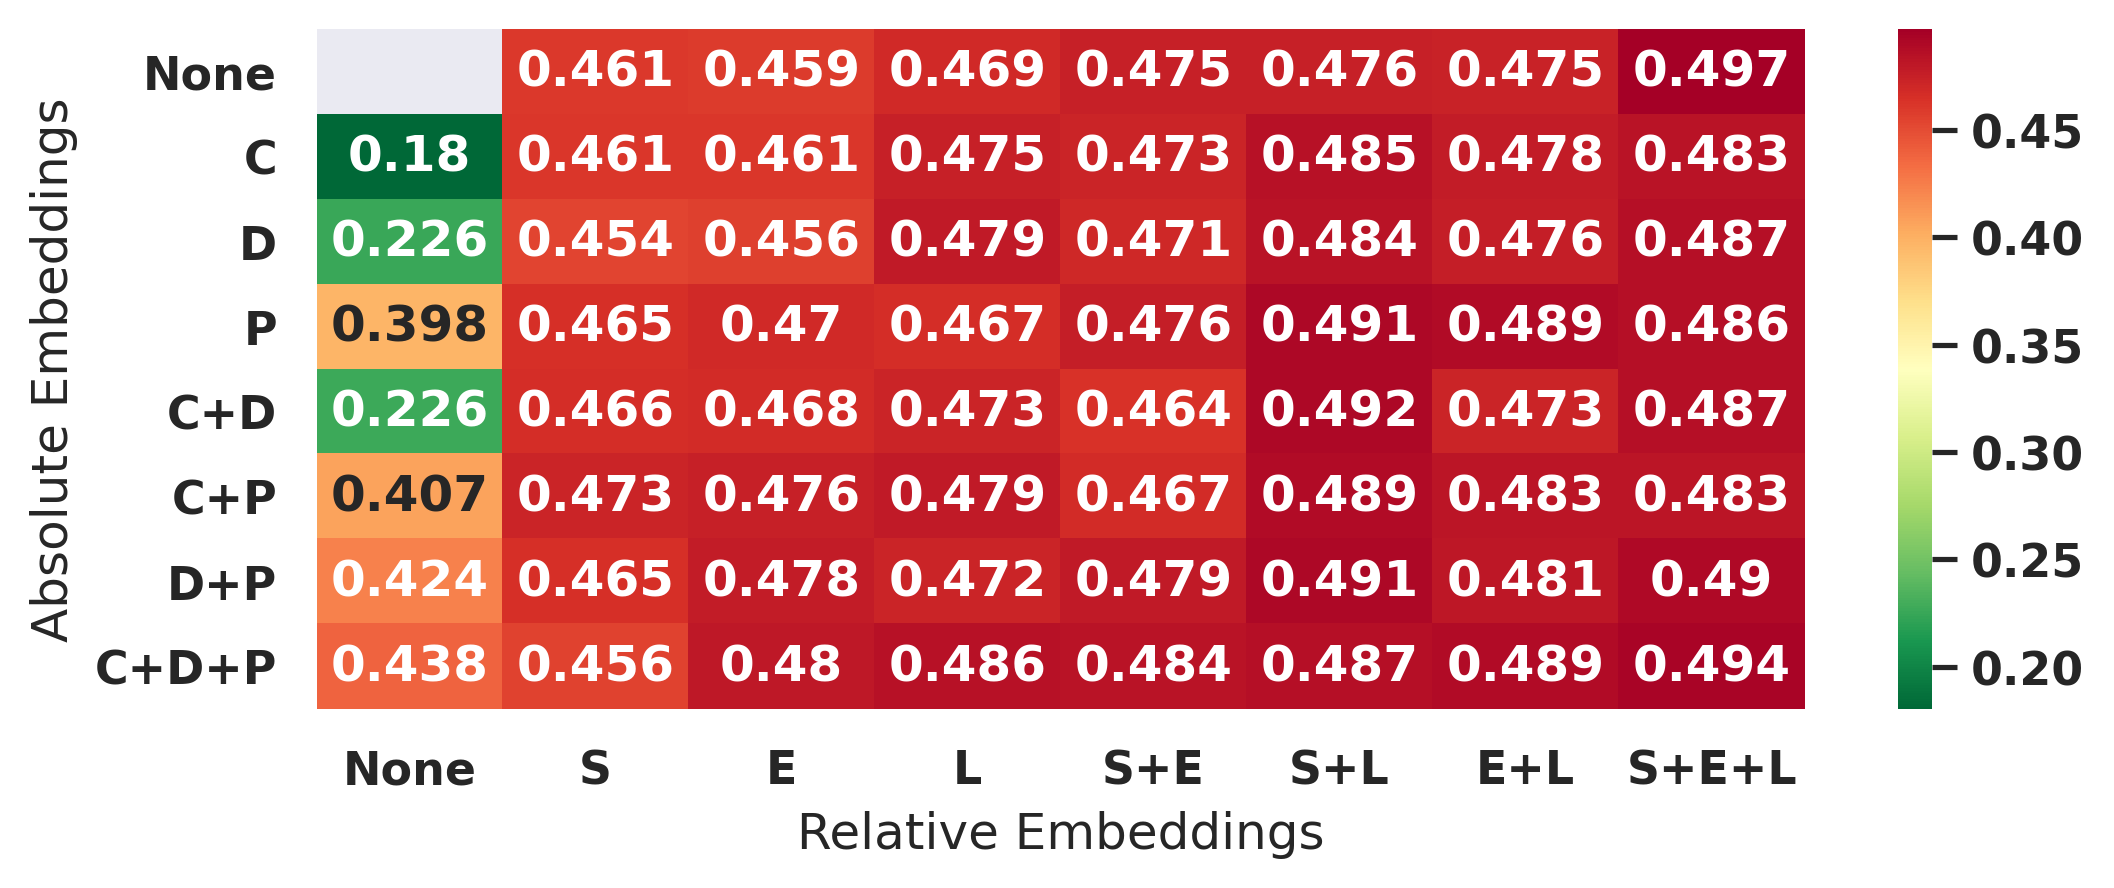
\includegraphics[width=\linewidth]{figures/combinations/ml-1m_60.png}
    %\caption{MovieLens 1M}
  \end{minipage}
  \begin{minipage}[t]{.49\linewidth}
    \centering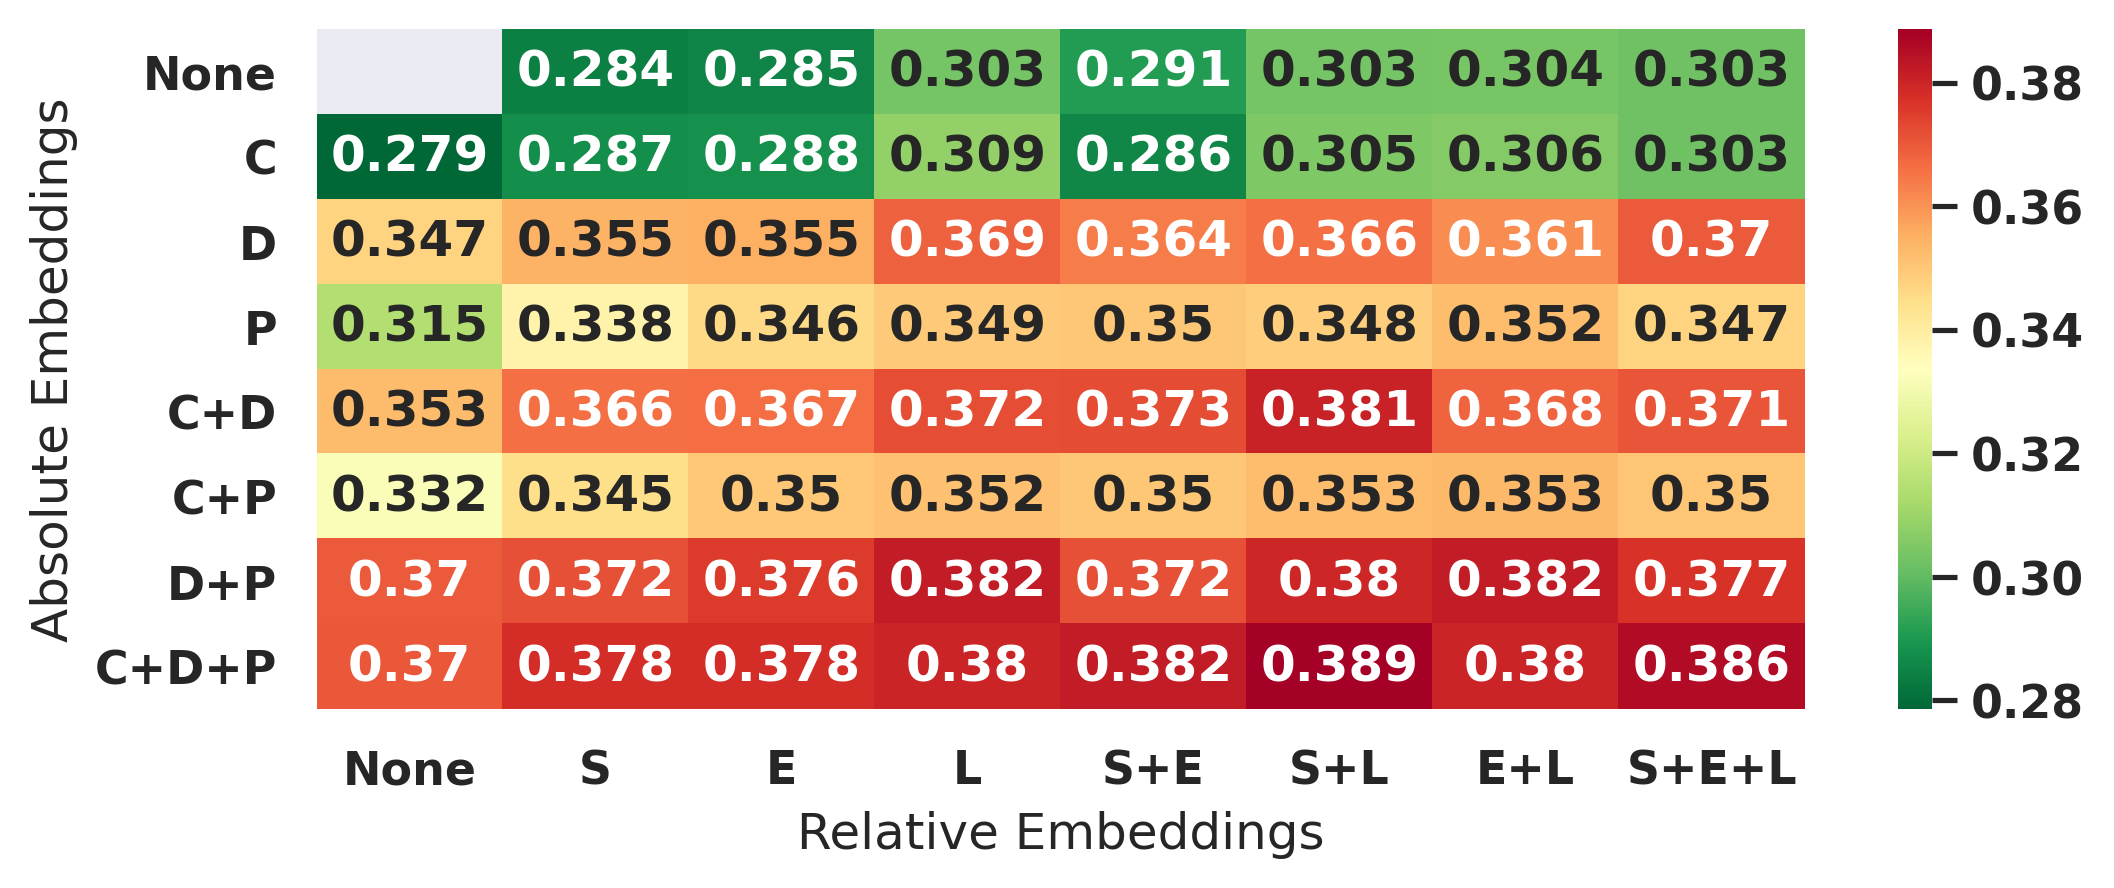
\includegraphics[width=\linewidth]{figures/combinations/game_60.png}
    %\caption{Amazon Game}
  \end{minipage}
  \caption{NDCG@10 Comparison with All Possible Combinations of Positional Embeddings on ML-1M (left) and Game (right) Dataset. C, D, P, S, E and L represent \textbf{Con}, \textbf{Day}, \textbf{Pos}, \textbf{Sin}, \textbf{Exp} and \textbf{Log}, repectively. We used $h=60$ for all experiments.}
  \Description[The figure describes heatmaps of NDCG@10 comparison with all possible combinations of embedding types on MovieLens 1M and Amazon Game]{The left figure is a heatmap of NDCG@10 comparison with all possible combinations of embedding types on MovieLens 1M. Absolute embeddings lie on y-axis and relative embeddings lie on x-axis. As we move further into the x-axis, the heatmap gets hotter. Columns with Log embedding seems to be the hottest. The right figure describes the same heatmap on Amazon Game. As we move further down on y-axis, the heatmap gets hotter. Rows with Day embedding seems to be the hottest.}
  \label{fig:tesearch}
\end{figure*}
Figure \ref{fig:tesearch} shows the comparison of all possible combinations of temporal embeddings on ML-1M and Amazon Game dataset. We fixed all other hyperparameters (e.g., $h=60$). Interestingly, the importance of each embedding seems to differ in each dataset. In ML-1M, relative position embeddings (especially \textbf{Log}) seem to play an important role, whereas in Amazon Game, absolute position embeddings (especially \textbf{Day}) seem to be essential. Therefore, the optimal combination is also different for each dataset. Further analysis with different $h$ shows us that while optimal combination differs slightly for each $h$, the overall tendency stays the same for each dataset. The same applies to other datasets. This suggests that datasets with distinct characteristics require carefully chosen temporal embeddings that provide the right views on the context of user-item interactions. Note that while we only used $n=2\text{ and }4$ for Table \ref{tab:results} to be fair with other baselines, using all possible $n$ can further improve our performance.
% EH: 아래와 같은 문장 정도면 어떨까 
%When we apply the same analysis on the different datasets, the best joint set of embeddings is different. According to our observation, each dataset has unique contextual characteristics which is useful information to predict the next behavior. 
%This suggests that datasets with different characteristics require different view on the positions of user-item interactions in a sequence. [ANALYZE WHY]

% In this section we seek to study the effect of various positional embeddings. To assess the contribution of each positional embedding type in more detail, we ran an extensive experiment to test all combinations of positional embeddings. Figure-\ref{fig:tesearch} shows the comparison of NDCG@10 performance on ML-1M and Amazon Game dataset. All other hyperparameters were kept equal.

% \begin{figure}[ht]
  \centering
  \begin{subfigure}[ht]{.49\linewidth}
    \centering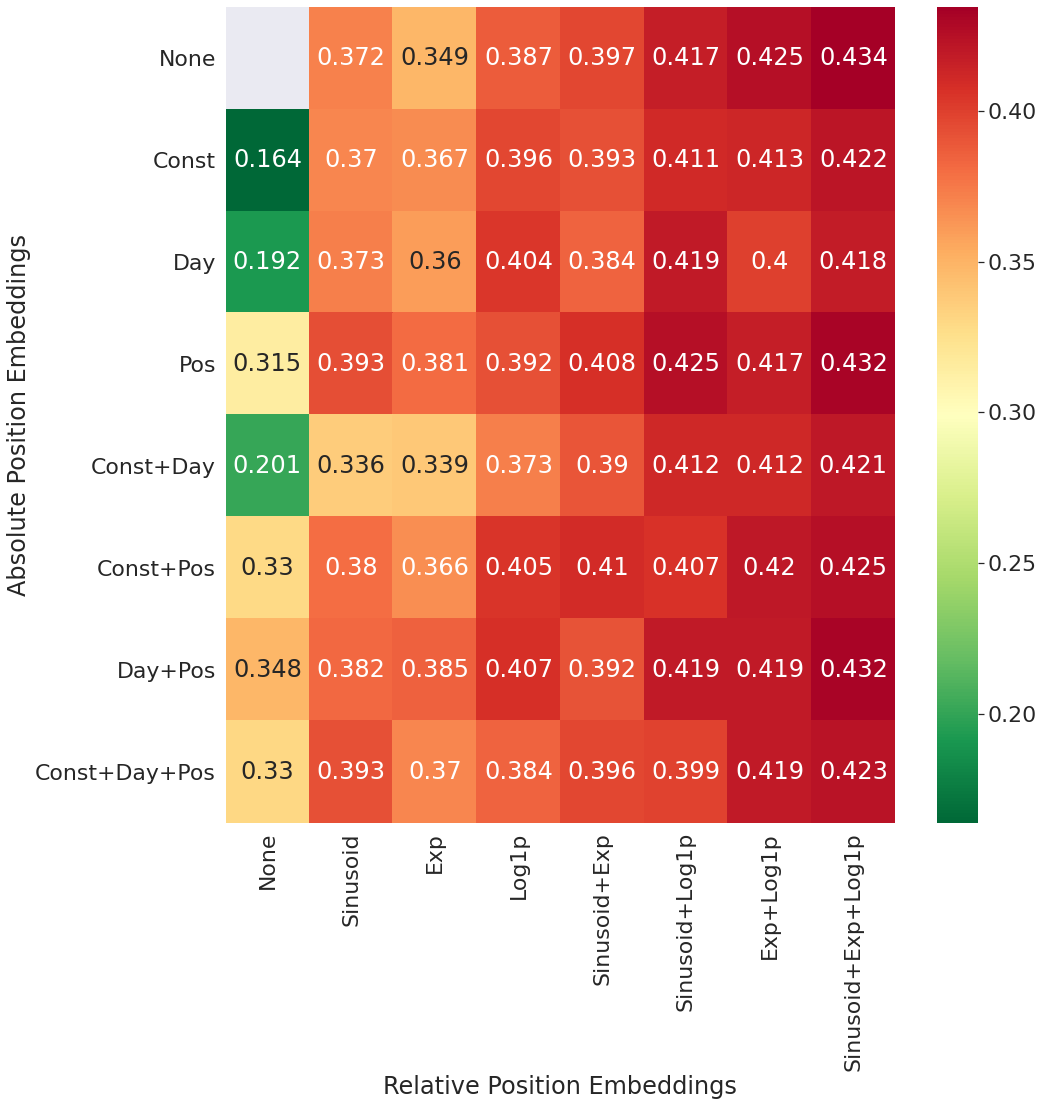
\includegraphics[width=.95\linewidth]{figures/tesearch.png}
    \caption{MovieLens 1M}
  \end{subfigure}
  \begin{subfigure}[ht]{.49\linewidth}
    \centering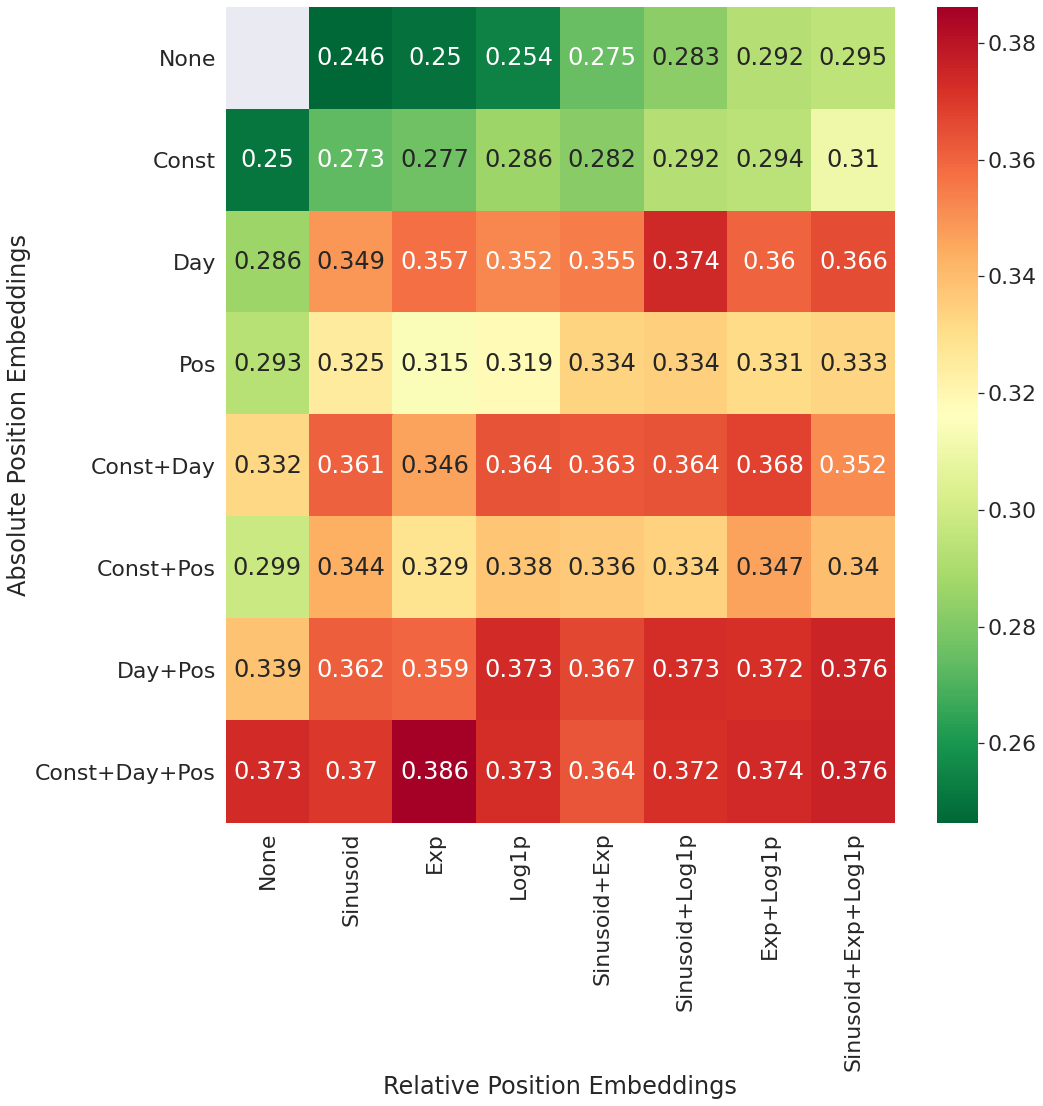
\includegraphics[width=.95\linewidth]{figures/tesearch_game.png}
    \caption{Amazon Game}
  \end{subfigure}
  \caption{NDCG@10 Comparison with All Possible Combinations of Positional Embeddings on ML-1M and Game Dataset}
  \Description{TODO:Description}
  \label{fig:tesearch}
\end{figure}

% Interestingly, the importance of each embedding seems to differ in each dataset. In ML-1M, relative position embeddings(especially \textbf{Log1p}) seem to play an important role, whereas in Amazon Game, absolute position embeddings(especially \textbf{Pos} and \textbf{Day}) seem to be essential. In ML-1M, the optimal performance is achieved when we use all three relative position embeddings and none of the absolute position embeddings. In contrast, using all three absolute position embeddings with only \textbf{Exp} relative embedding works best in Amazon Game. This proves that datasets with different characteristics require different view on the positions of user-item interactions in a sequence.

% %\begin{figure}[ht]
  \centering
  
  \begin{subfigure}[ht]{.33\linewidth}
    \centering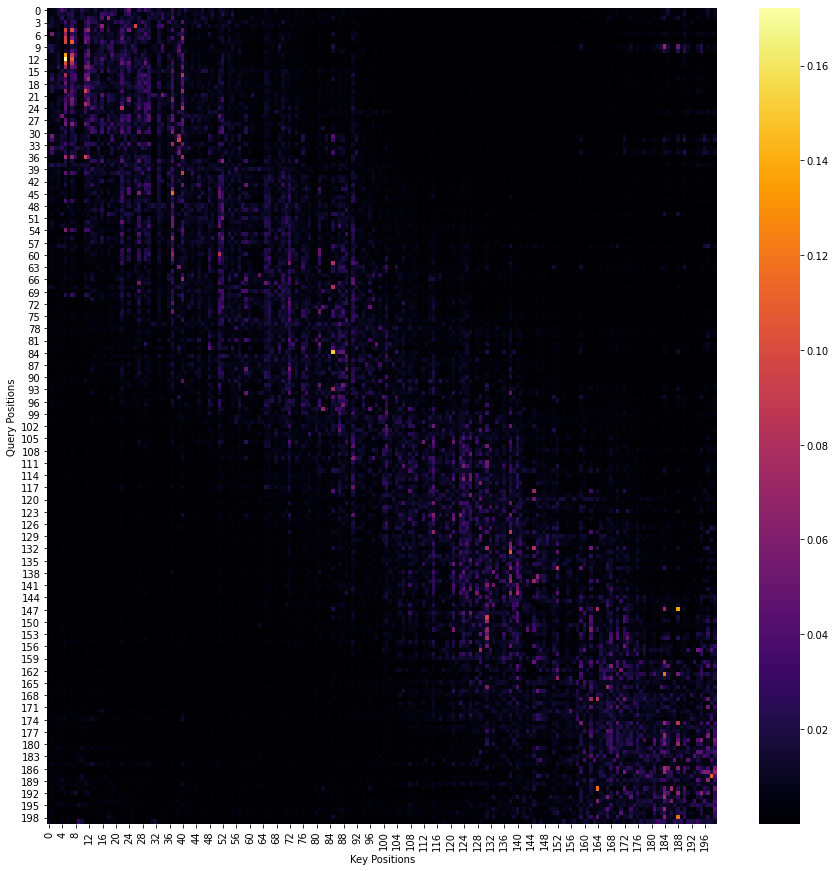
\includegraphics[width=.95\linewidth]{figures/attn1/L0BPH1.png}
    \caption{\textbf{Pos} Layer 0 Head 1}
  \end{subfigure}
  \begin{subfigure}[ht]{.33\linewidth}
    \centering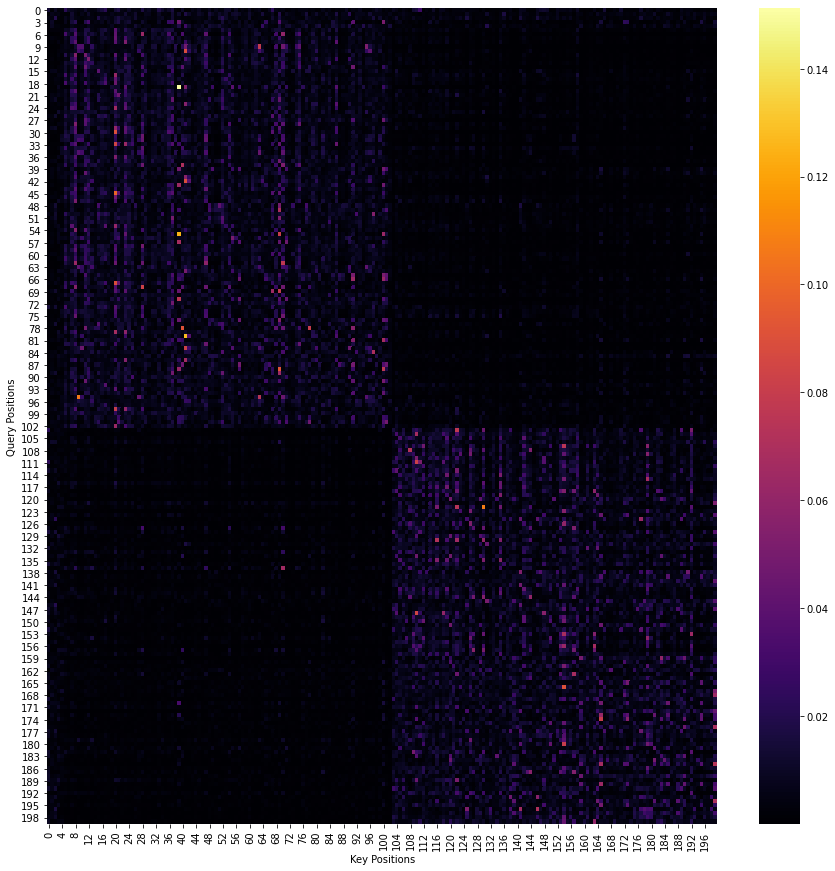
\includegraphics[width=.95\linewidth]{figures/attn1/L0BDH0.png}
    \caption{\textbf{Day} Layer 0 Head 0}
  \end{subfigure}
  \begin{subfigure}[ht]{.33\linewidth}
    \centering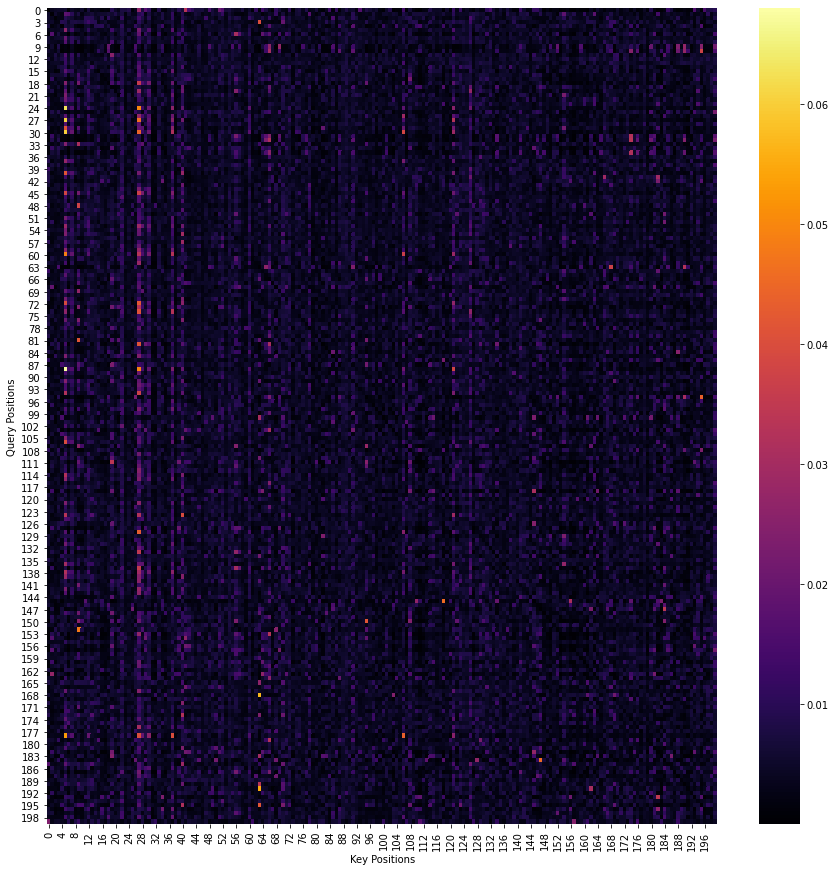
\includegraphics[width=.95\linewidth]{figures/attn1/L0BCH0.png}
    \caption{\textbf{Const} Layer 0 Head 0}
  \end{subfigure}
  \begin{subfigure}[ht]{.33\linewidth}
    \centering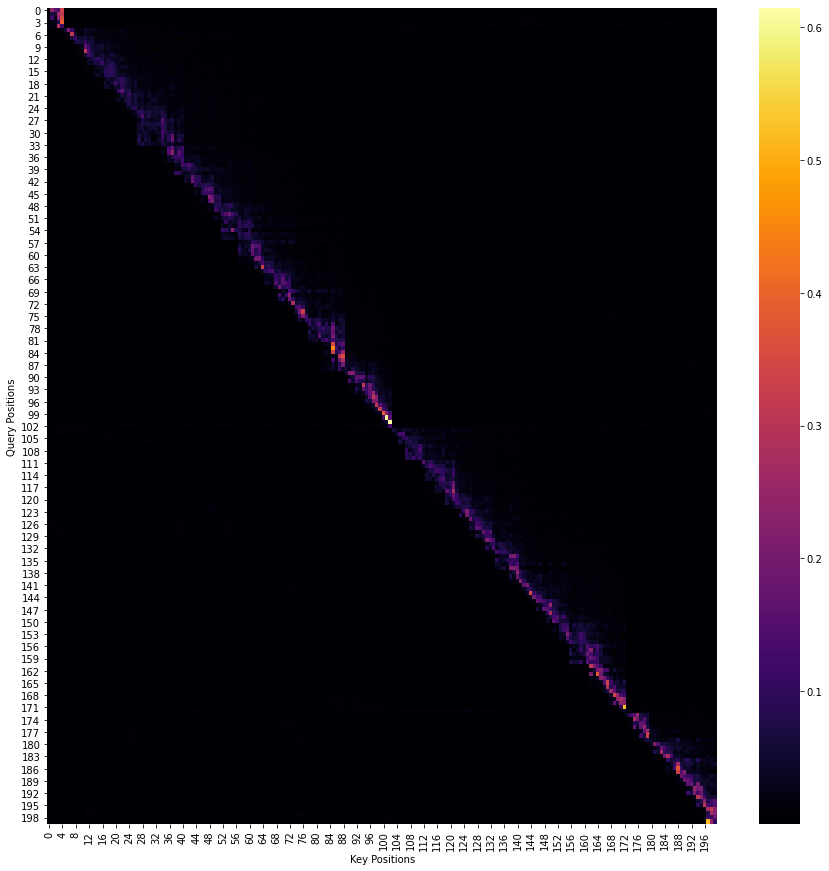
\includegraphics[width=.95\linewidth]{figures/attn1/L0BSH0.png}
    \caption{\textbf{Sinusoid} Layer 0 Head 0}
  \end{subfigure}
  \begin{subfigure}[ht]{.33\linewidth}
    \centering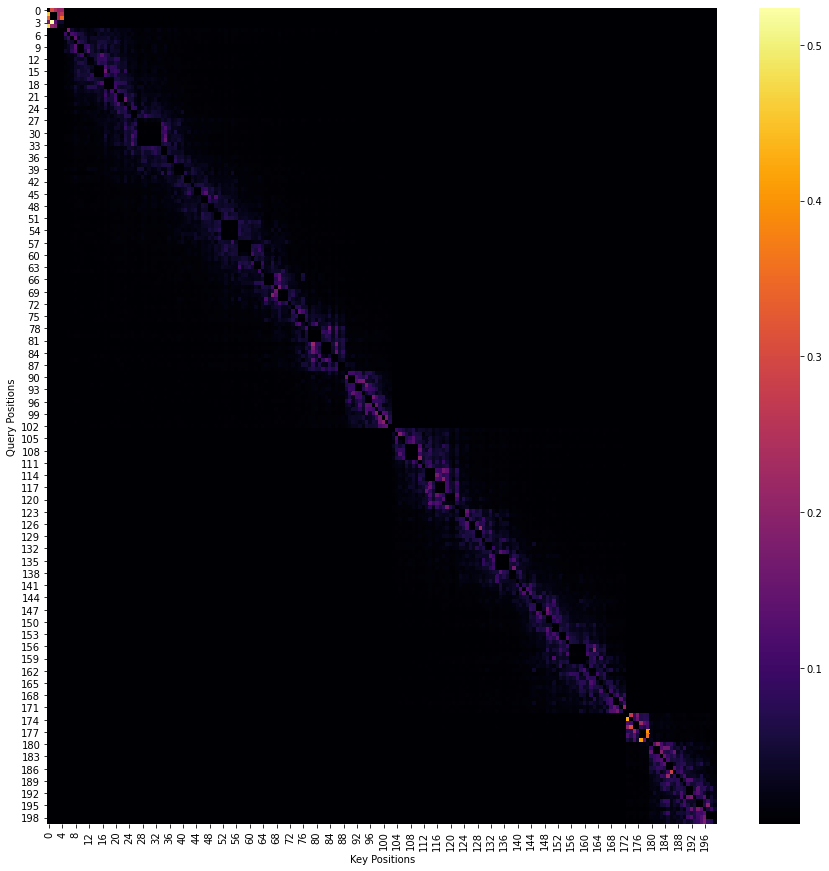
\includegraphics[width=.95\linewidth]{figures/attn1/L0BEH0.png}
    \caption{\textbf{Exp} Layer 0 Head 0}
  \end{subfigure}
  \begin{subfigure}[ht]{.33\linewidth}
    \centering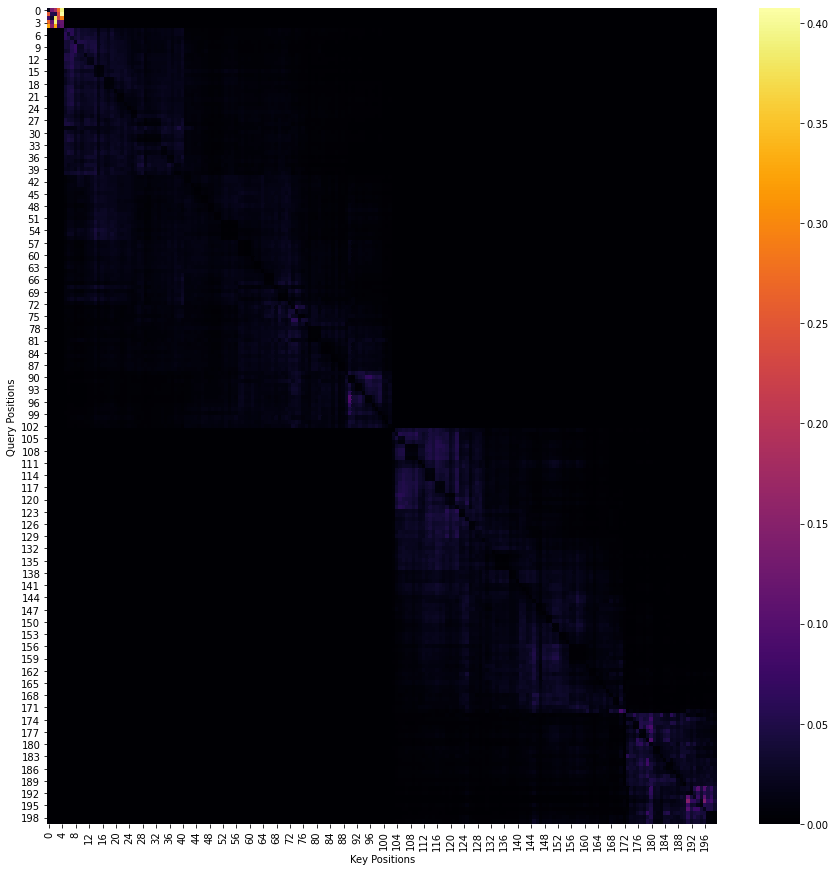
\includegraphics[width=.95\linewidth]{figures/attn1/L1BLH0.png}
    \caption{\textbf{Log1p} Layer 1 Head 0}
  \end{subfigure}
  
  %\subfigure{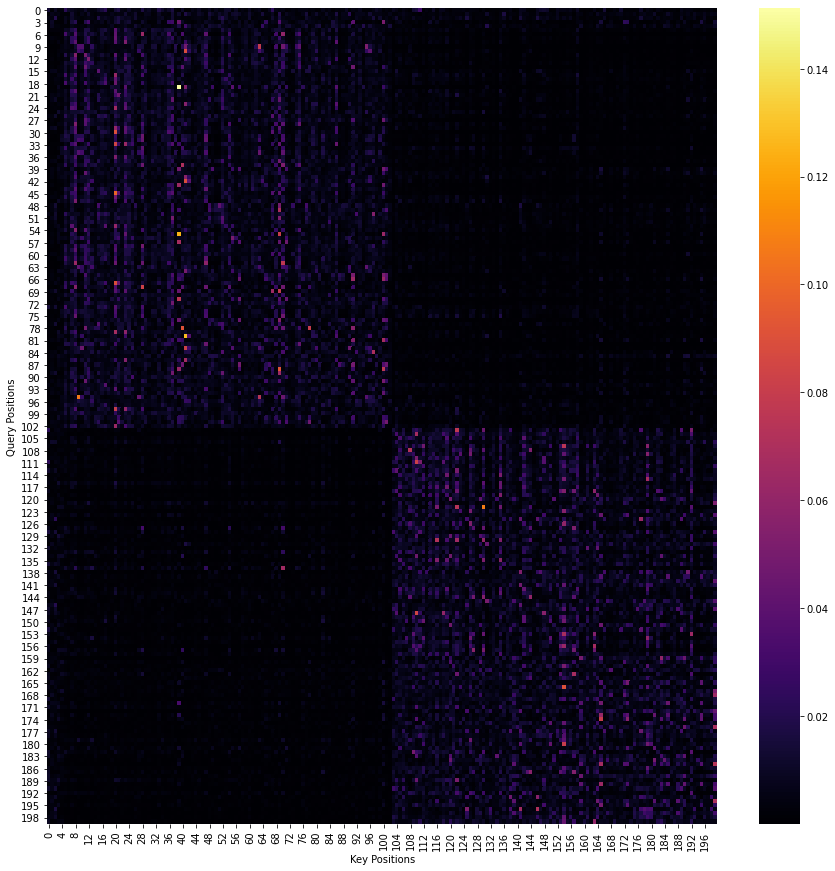
\includegraphics[width=0.5\linewidth]{figures/attn1/L0BDH0.png}}
  %\subfigure{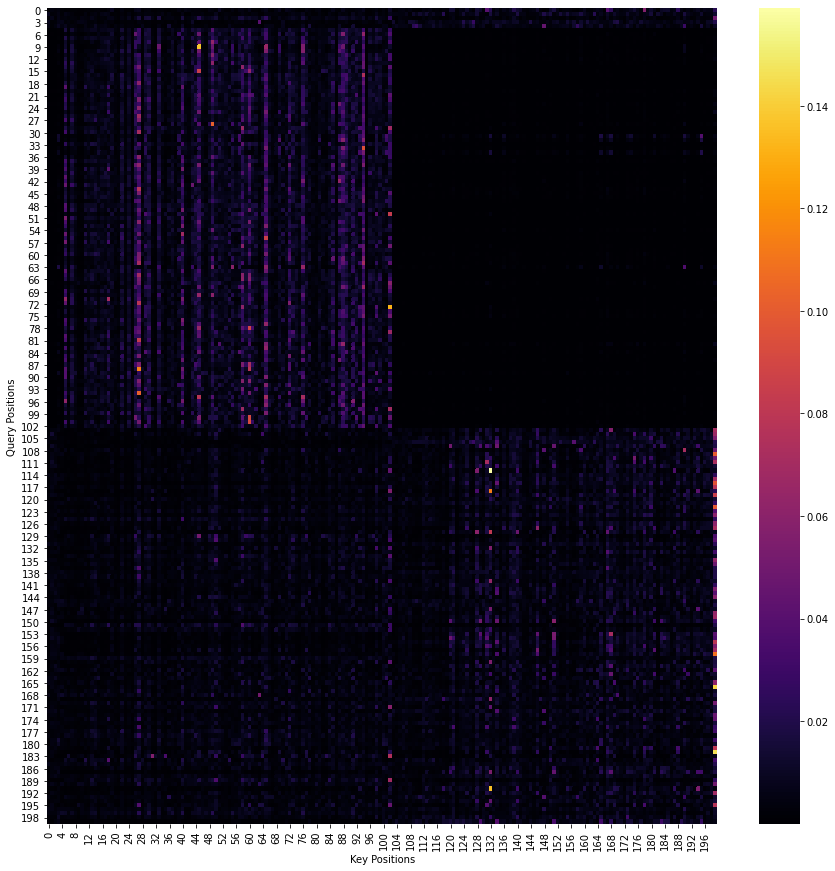
\includegraphics[width=0.5\linewidth]{figures/attn1/L0BDH1.png}}
  \caption{Attention Score Maps (Might need to change the figures to ones with shorter sequences (so that they are more clear))}
  \Description{TODO:Description}
  \label{fig:attnmaps}
\end{figure}

% \begin{table}[ht]
\caption{Gradient Comparison for Each Embedding Type}
\label{tab:grad_cam}
\begin{tabular}{@{}lllllll@{}}
\toprule
{Dataset} & {Pos}           & {Day}              & {Const}            & {Sinusoid}         & {Exp}           & {Log1p}         \\ \midrule
{ML1M}    & {4.79\%}        & {5.34\%}           & {1.50\%}           & {\textbf{51.34\%}} & {7.08\%}        & {\underline{29.94\%}} \\
{ML20M}   & {\underline{19.60\%}} & {5.50\%}           & {6.11\%}           & {\textbf{24.51\%}} & {\underline{22.58\%}} & {\underline{21.70\%}} \\
{Beauty}  & {1.03\%}        & {8.39\%}           & {\textbf{57.12\%}} & {9.79\%}           & {0.69\%}        & {\underline{22.98\%}} \\
{Game}    & {\underline{40.39\%}} & {\textbf{49.57\%}} & {1.96\%}           & {1.19\%}           & {1.37\%}        & {5.51\%}  \\ \bottomrule
\end{tabular}
\end{table}

% To further measure the contributions of each embedding type, we applied a method similar to Grad-CAM\cite{GRADCAM} to our fully equipped model(with all 6 embedding types). For every sequence in the test data, we took the output from the final layer of our self-attention block stacks $\mathbf{Z}^L = [\mathbf{Z}^L_1, ..., \mathbf{Z}^L_\Sigma]$, and then computed the gradient of each output with regard to the answer item's logit $y^c$:
% \begin{equation}
%     g_i = \frac{dy^c}{dZ^L_i}
% \end{equation}
% Similar to \cite{GRADCAM}, we only took positive gradients from $g_i$ to measure their positive influence on the answer's logit. We calculated the average of their sums and then applied softmax to get Table-\ref{tab:grad_cam}.

% As we expected, relative position embeddings were dominant in MovieLens datasets, while absolute position embeddings were dominant in Amazon datasets. Moreover, as we saw in Figure-\ref{fig:tesearch}-(b), \textbf{Pos} and \textbf{Day} play very important roles in Amazon Game. Unlike Figure-\ref{fig:tesearch}-(a), \textbf{Sinusoid} seems to be more influential than \textbf{Log1p} in ML-1M. However, it is interesting to note that \textbf{Log1p} stays somewhat influential throughout all datasets. Another interesting observation is the dominance of \textbf{Const} in Amazon Beauty. This seems to suggest that positional bias is relatively less important in Amazon Beauty dataset. These results show that one must carefully design the positional embeddings in the recommendation system by considering the characteristics of the dataset.

% %Due to limited space, we study the images of attention score maps for each embedding type in Appendix-\ref{app:attnmaps}.

% %Figure-\ref{fig:attnmaps} shows the attention score maps for different positional embeddings. Due to limited space, we only present representative maps. We provide full-scope attention maps in Appendix-

% %(Analysis on Figure-\ref{fig:attnmaps})


%\subsection{Effect of Multi Self-attention Blocks}
%Although we let all transformer-based models have the same number of layers and heads in our experiments, MEANTIME has more parameters than SASRec, TiSASRec, and BERT4Rec since it employs 6 self-attention blocks per layer in contrast to 1. This might seem unfair since the performance gain could have come from the larger parameter size, or from the multi-path self-attention. To prove that this is not the case, we also experimented with the adjusted baseline models where they also have 6 self-attention blocks per layer. We call them \textbf{buffed} models. 

\begin{table}[h]
\caption{Performance Comparison with Buffed Baselines.}
\label{tab:buff_results}
\begin{tabular}{@{}lrrrrr@{}}
\toprule
{Metrics} & {SASRec-Buffed}& {TiSASRec-Buffed} & {BERT4Rec-Buffed} & {MEANTIME}      \\ \midrule
{Recall@5}  & {0.5512} & {0.5528} & {0.5916} & {\textbf{0.6154}} \\
{Recall@10}  & {0.6853} & {0.6856} & {0.6987} & {\textbf{0.7268}} \\
{NDCG@5}   & {0.3955} & {0.3962}  & {0.4437} & {\textbf{0.4690}} \\
{NDCG@10}  & {0.4390} & {0.4393}  & {0.4785} & {\textbf{0.5052}} \\ \bottomrule
\end{tabular}
\end{table}

Table-\ref{tab:buff_results} shows the comparison results. All experiments were done with ML-1M dataset, hidden dimension size $h=64$, dropout ratio 0.2 and weight decay 0. The result clearly shows that the strong performance of MEANTIME does not merely come from large parameter size nor multi-path self-attention.

%\subsection{Effect of Information Separation}

%\subsection{Effect of Hidden Dimension Size}
%Here we study the effect of hidden dimension size on each dataset. We experiment with $h \in \{16, 32, 64, 128\}$ while keeping other hyperpameters the same.

\begin{figure}[ht]
  \centering
  
  \begin{subfigure}[ht]{\linewidth}
    \centering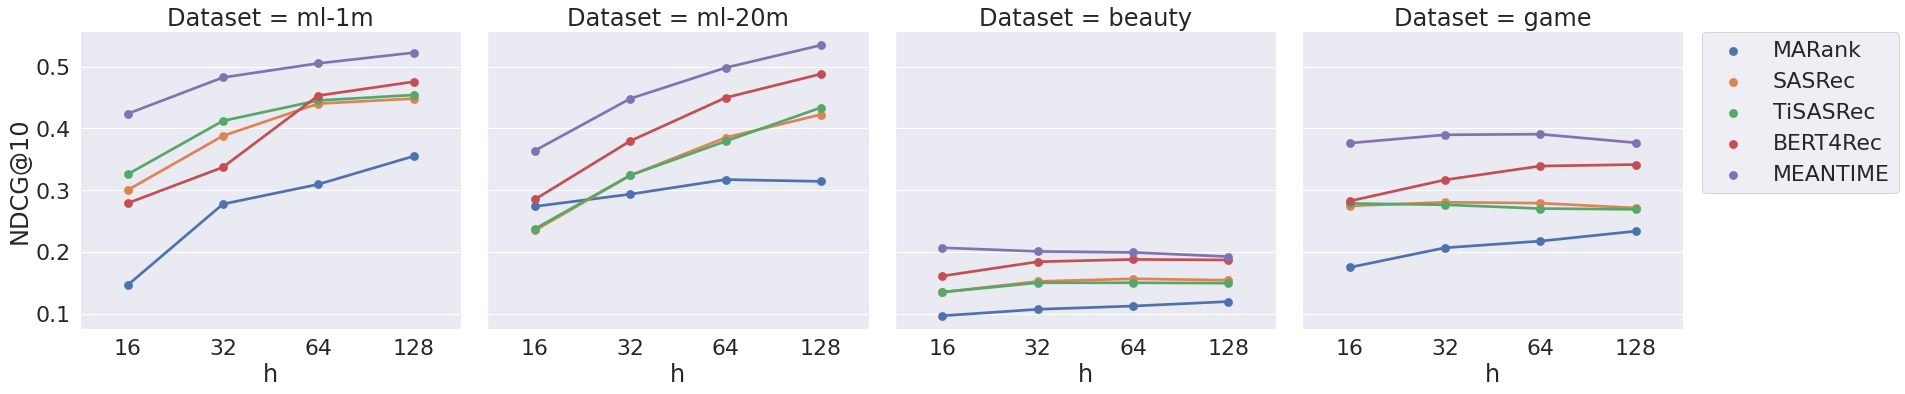
\includegraphics[width=\linewidth]{figures/impact_h/n10.png}
    \caption{NDCG@10}
  \end{subfigure}
  \begin{subfigure}[ht]{\linewidth}
    \centering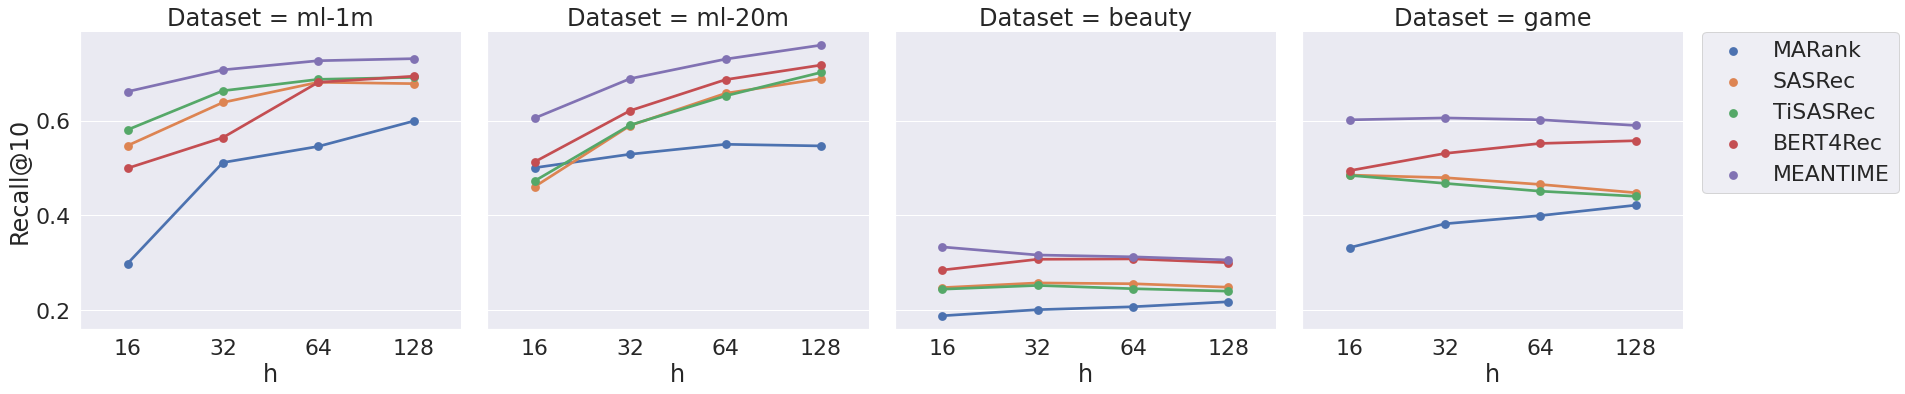
\includegraphics[width=\linewidth]{figures/impact_h/r10.png}
    \caption{Recall@10}
  \end{subfigure}
  
  \caption{Effect of hidden dimension size on NDCG@10 and Recall@10}
  \Description{TODO:Description}
  \label{fig:himpact}
\end{figure}

Figure-\ref{fig:himpact} shows the comparison results. We observe that optimal hidden dimension size differs between datasets. Interestingly, MEANTIME works optimally at $h = 16$ in Amazon Beauty dataset. This is probably because it is the most sparse dataset of the four, which makes it prone to overfitting.

We also observe that without extensive hyperparameter tuning, TiSASRec\cite{TISASRec}, which uses temporal infromation to improve SASRec\cite{SASRec}, sometimes doesn't outperform SASRec. In contrast, MEANTIME, which improves BERT4Rec\cite{BERT4Rec} with temporal information, always outperforms BERT4Rec (and all other baseline models) even without parameter tuning. This seems to prove the superiority of our model. [TOO MUCH BRAGGING?]

%\subsection{Effect of freq \& $\tau$}
%\begin{figure}[ht]
  \centering
  \begin{subfigure}[ht]{.45\linewidth}
    \centering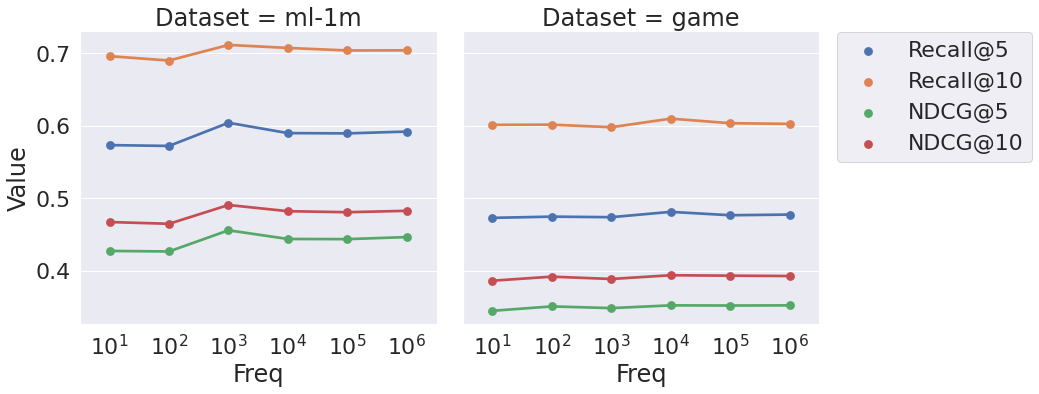
\includegraphics[width=\linewidth]{figures/freq_tau/freq_search.png}
    \caption{Effect of \textit{freq}}
  \end{subfigure}
  \begin{subfigure}[ht]{.45\linewidth}
    \centering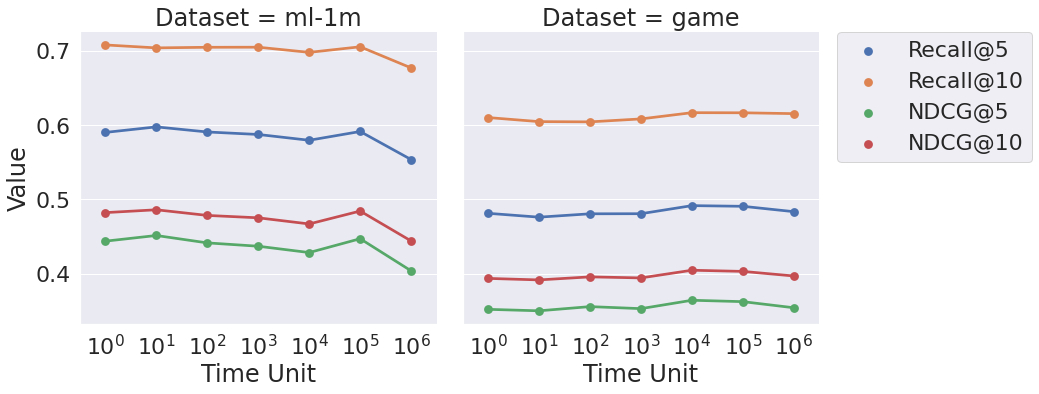
\includegraphics[width=\linewidth]{figures/freq_tau/tau_search.png}
    \caption{Effect of $\tau$}
  \end{subfigure}
  \caption{Effect of \textit{freq} and $\tau$ on performance}
  \Description{TODO:Description}
  \label{fig:freq_tau}
\end{figure}

%% CONCLUSION
\section{Conclusion}
In this paper we presented MEANTIME, which uses time information and multiple encoding functions to provide distinctive positional embeddings to self-attention modules.  Experiments on four real-world datasets show that our model outperforms state-of-the-art baselines in sequential recommendation. Through extensive ablation study, we also showed that different datasets require different positional embeddings to gain optimal performance. This suggests that one must carefully tune the positional factor in their model considering the characteristics of their own dataset.
%Although our intention was to explore the vast possibility of temporal encoding functions, we acknowledge that the choice of our encoding functions might seem too improvised. We plan to investigate a more general form of embedding that can automatically adjust to the dataset in the future.


\begin{acks}
This work was supported by Samsung Electronics and the National Research Foundation of Korea (NRF) grant (PF Class Heterogeneous High Performance Computer Development, NRF-2016M3C4A7952587) funded by the Ministry of Science, ICT \& Future Planning (No. 2013R1A3A2003664).
\end{acks}


%% ACKNOWLEDGEMENTS
%\begin{acks}
%Acknowledgements.
%\end{acks}

%%
%% The next two lines define the bibliography style to be used, and
%% the bibliography file.
\bibliographystyle{ACM-Reference-Format}
\bibliography{bibs}
%% Appendix
%\appendix
%\section{General Temporal Embedding With Fourier Series}
%\input{sections/appendix_A}

%\section{Full-scope Attention Maps}
%\input{sections/appendix_B}

\end{document}
\endinput

%% End of file `sample-manuscript.tex'.
